\documentclass[fr]{../../../eplsummary}

\usepackage[minted]{../../../eplcode}
\usepackage{../../../eplunits}
\usepackage{interval}
\usepackage{tikz}
\usetikzlibrary{calc,patterns,angles,quotes}
\usepackage{pgfplots}
\pgfplotsset{compat=1.15}
\usepackage{float}
\usepackage{bm}
\usepackage{wrapfig}
\usepackage{multicol}
\usepackage{mathrsfs}

\newcommand{\Rnm}{\R^{n \times m}}
\newcommand{\Tin}{T_{\textnormal{in}}}
\newcommand{\barTin}{\bar{T}_{\textnormal{in}}}
\newcommand{\kp}{k_{\textnormal{p}}}
\newcommand{\taui}{\tau_{\textnormal{i}}}
\newcommand{\taud}{\tau_{\textnormal{d}}}
\newcommand{\xaug}{x_{\textnormal{aug}}}
\newcommand{\Aaug}{A_{\textnormal{aug}}}
\newcommand{\laplacian}{\mathscr{L}}
\newcommand{\commandability}{\mathcal{C}}
\newcommand{\observability}{\mathcal{O}}
\newcommand{\omegap}{\omega_{\textnormal{p}}}
\newcommand{\Gjw}{G(\imagj \omega)}
\newcommand{\Geq}{G_{\textnormal{eq}}}
\newcommand{\phasem}{\phi_{\textnormal{m}}}
\newcommand{\gainm}{G_\textnormal{m}}

\renewcommand{\Re}{\mathrm{Re}}

\DeclareSIUnit{\dec}{decade}

\DeclareMathOperator{\numerator}{num}
\DeclareMathOperator{\denominator}{den}
\DeclareMathOperator{\adj}{adj}
\DeclareMathOperator{\rank}{rank}

% TODO disparité fiche eq 5.3/slide 71
% TODO fix legend dans rep indicielle
% TODO fix axes dans bode

\hypertitle[']{Automatique linéaire}{6}{INMA}{1510}
{Gilles Peiffer}
{Denis Dochain}

\section{Représentation d'état}
\subsection{Représentation d'état des systèmes linéaires}
\begin{mydef}
	Un \emph{système linéaire à temps invariant} de dimension $n \in \N$
	est décrit par un système d'équations différentielles ordinaires
	linéaires formulées sous forme matricielle comme suit:
	\begin{equation}
		\label{eq:ssrep}
		\left\{
		\begin{array}{rcl}
			\dot{x}(t) & = & Ax(t) + Bu(t) + Dv(t)\,, \\
			      y(t) & = & Cx(t)\,,
		\end{array}
		\right.
	\end{equation}
	avec $A \in \R^{n \times n}$ la matrice d'état
	et $x(t) \in \R^n$ l'état,
	$B \in \R^{n \times p}$ la matrice d'entrée de commande
	et $u(t) \in \R^p$ l'entrée de commande,
	$D \in \R^{n \times d}$ la matrice d'entrée de perturbation
	et $v(t) \in \R^d$ l'entrée de perturbation,
	$C \in \R^{m \times n}$ la matrice de sortie
	et $y(t) \in \R^m$ la sortie.
	On a en général $y(t) = Cx(t)$, sans terme en $u$,
	car celui-ci rendrait le système non causal.
	Tout système physique est causal.
	On peut en général écrire ce système comme
	\begin{equation}
		\label{eq:ssgen}
		\left\{
		\begin{array}{rcl}
			\dot{x}(t) & = & f\big(x(t), u(t), v(t)\big)\,, \\
			      y(t) & = & h\big(x(t)\big)\,,
		\end{array}
		\right.
	\end{equation}
	La fonction \matlab{} \mintinline{matlab}{ss}
	permet d'obtenir la représentation d'état d'un système continu,
	cependant d'une forme légèrement différente:
	\begin{align}
		\dot{x} &= Ax + Bu\,, \notag \\
		y &= Cx + Du\,. \notag
	\end{align}
\end{mydef}
\begin{mydef}
	La représentation d'état est sujette au vocabulaire suivant.
	\begin{itemize}
		\item Le \emph{polynôme caractéristique} en boucle fermée
		est défini par le polynôme en $s$ suivant: $\det(sI - A)$.
		Cette variable $s$ est la \emph{variable fréquentielle}.
		\item Les \emph{modes} ou \emph{pôles} du système
		sont les solutions de l'équation caractéristique,
		$\det(sI - A) = 0$.
		\item Les pôles à partie réelle strictement négative
		sont dits \emph{stables},
		ceux à partie réelle positive sont \emph{instables}.
	\end{itemize}
\end{mydef}

Lorsqu'on a la représentation d'état (\ref{eq:ssrep}),
et qu'on utilise la commande proportionnelle-intégrale,
on a la relation (\ref{eq:sspi}).
On peut alors définir un vecteur d'état augmenté $\xaug$
et une matrice $\Aaug$ comme suit:
\begin{equation}
	\xaug \coloneqq \begin{pmatrix} x \\ \frac{\kp}{\taui} \int_0^t (y^* - y) \dif \tau \end{pmatrix} \implies \Aaug \coloneqq \begin{pmatrix} A & \frac{\kp}{\taui} \\ CA & 0 \end{pmatrix}\,.
\end{equation}

\subsection{Commande de systèmes}
Le but de ce cours est de trouver comment commander un système,
c'est-à-dire comment agir sur certaines variables du système
de manière à assurer un comportement désiré en dépit de perturbations.

\subsubsection{Synthèse d'une loi de commande}
La synthèse d'une loi de commande se fait en plusieurs étapes.
On s'intéresse toujours au comportement dynamique en boucle fermée.
\paragraph{Détermination de l'équilibre}
L'\emph{équilibre} est la situation où $\dot{x} = 0$,
c'est-à-dire qu'on cherche les points où $x = \bar{x}$,
solution de $A \bar{x} + B \bar{u} + D \bar{v} = 0$
pour un jeu de valeurs $(\bar{u}, \bar{v})$.

Cette équation a une solution simple si $A$ est de plein rang,
provenant du fait que $Ax = b \iff x = A^{-1}b$.
\begin{equation}
	\bar{x} = -A^{-1}B \bar{u} - A^{-1} D \bar{v}\,.
\end{equation}

\begin{mytheo}
	Travailler avec la variable originale $x$
	est équivalent à travailler avec
	la variable variationnelle $\tilde{x} = x - \bar{x}$
	dans le cadre des systèmes linéaires.
\end{mytheo}
\begin{proof}
	\begin{align*}
		\dot{x} &= Ax + Bu + Dv \\
		&= A (\tilde{x} + \bar{x}) + B (\tilde{x} + \bar{x}) + D (\tilde{x} + \bar{x}) \\
		&= A \tilde{x} + B \tilde{x} + D \tilde{x} + \underbrace{A \bar{x} + B \bar{x} + D \bar{x}}_{0 \textnormal{ par déf. équilibre}} \\
		&= A \tilde{x} + B \tilde{x} + D \tilde{x} \\
		&= \dot{\tilde{x}}\,.\qedhere
	\end{align*}
\end{proof}

\paragraph{Commande proportionnelle (P)}
On rajoute ensuite la commande proportionnelle,
qui permet de corriger le signal.
On définit l'erreur comme $e = y^* - y$.
La commande proportionnelle est alors
\begin{equation}
	\label{eq:pcontrol}
	u = u^* + \kp (y^* - y)\,,
\end{equation}
avec $u^* = \bar{u}$ et $y^* = \bar{y}$.
La constante $\kp > 0$ est le \emph{gain du régulateur}.
On distingue deux cas:
\begin{itemize}
	\item Si $y = y^*$, on se trouve dans le cas idéal
	et l'erreur de commande tend vers zéro quand $t$ augmente:
	$\lim_{t \to +\infty} e(t) = 0$.
	\item Si $y \ne y^*$, l'équation différentielle pour trouver l'erreur
	n'est plus inconditionnellement stable.
\end{itemize}

\paragraph{Commande proportionnelle-intégrale (PI)}
En plus de la commande proportionnelle,
on rajoute un commande intégrale
avec une constante de temps d'intégration $\taui > 0$ comme
\begin{equation}
	\label{eq:sspi}
	u = u^* + \kp (y^* - y) + \frac{\kp}{\taui} \int_0^t (y^* - y) \dif \tau\,.
\end{equation}
Cet intégrateur permet d'\og absorber \fg{} la variation de la perturbation.
À l'équilibre, on a
\begin{equation}
	\label{eq:pierr}
	\fdif{e}{t} = \fdif{}{t} \left( \int_0^t (y^* - y) \dif \tau \right) = 0 \implies e = 0\,.
\end{equation}
Cette implication découle du fait que
comme on travaille avec des grandeurs variationnelles,
les conditions initiales sont nulles.

\begin{myexem}
	On illustre par l'exemple d'une cuve parfaitement mélangée en continu,
	montrée en \figuref{cuve}.
	Le but est de maintenir la température dans la cuve à une valeur désirée
	en agissant sur la puissance de chauffage de l'échangeur de chaleur,
	et ce en dépit de variations de la température d'entrée.
	\begin{figure}[H]
		\centering
		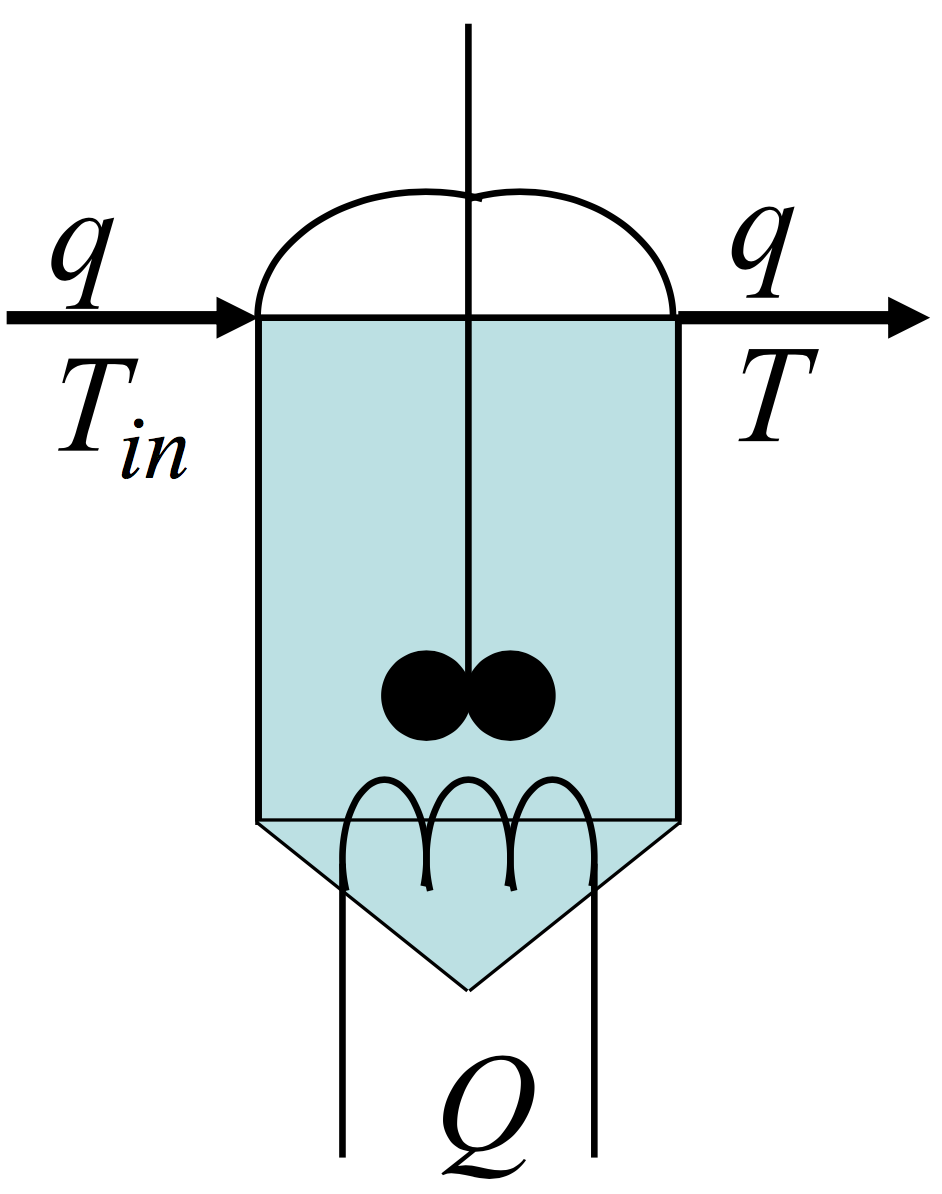
\includegraphics[width=0.2\textwidth]{img/cuve}
		\caption{Vue schématique de la cuve parfaitement mélangée.}
		\label{fig:cuve}
	\end{figure}
	L'équation de bilan thermique est
	\begin{equation}
		\fdif{T}{t} = \frac{q}{V}(\Tin - T) + \frac{1}{\rho C_{\textnormal{p}} V} Q\,.
	\end{equation}
	On voit que $T$ est la variable commandée,
	$T_{\textnormal{in}}$ est la variable de perturbation et
	$Q$ est la variable de commande.

	La synthèse d'une loi de commande se fait en plusieurs étapes.
	\paragraph{Détermination de l'équilibre}
	On cherche les valeurs de $T$ qui,
	pour un jeu de valeurs $(Q, \Tin)$,
	sont solutions de $\fdif{T}{t} = 0$, c'est-à-dire de
	\begin{align*}
		\frac{q}{V} (\barTin - \bar{T}) + \frac{1}{\rho C_{\textnormal{p}} V} \bar{Q} &= 0 \\
		\iff \bar{T} &= \barTin + \frac{1}{\rho C_{\textnormal{p}}q} \bar{Q}\,.
	\end{align*}
	\paragraph{Commande proportionnelle}
	On obtient immédiatement
	en remplaçant les variables dans (\ref{eq:pcontrol}) que
	\[
	Q = \bar{Q} + \kp (\bar{T} - T)\,.
	\]
	On vérifie bien que dans le premier cas
	(la première égalité est vraie car $e = \bar{T} - T$)
	\begin{align*}
	\fdif{e}{t} &= -\fdif{T}{t} = -\frac{q}{V} \left(\Tin - T + \bar{T} - \bar{T} \right) - \frac{1}{\rho C_{\textnormal{p}} V} \left( \bar{Q} + \kp (\bar{T} - T)\right) \\
	\iff \fdif{e}{t} &= -\left[ \frac{q}{V} + \frac{\kp}{\rho C_{\textnormal{p}} V} \right] e \implies \lim_{t \to +\infty} e(t) = 0
	\end{align*}
	alors que dans le deuxième cas,
	\[
	\fdif{e}{t} = -\left[ \frac{q}{V} + \frac{\kp}{\rho C_{\textnormal{p}} V} \right] e - \frac{q}{V} (\Tin - \barTin) \implies \lim_{t \to +\infty} e(t) = \frac{\dfrac{q}{V} (\barTin - \Tin)}{\dfrac{q}{V}+\dfrac{\kp}{\rho C_{\textnormal{p}}V}} \ne 0\,.
	\]
	\paragraph{Commande proportionnelle-intégrale}
	On remplace dans (\ref{eq:sspi}) pour trouver
	\[
	Q = \bar{Q} + \kp (\bar{T} - T) + \frac{\kp}{\taui} \int_0^t (\bar{T} - T) \dif \tau\,.
	\]
	On confirme bien que $\dif e/\dif t = 0$, comme en (\ref{eq:pierr}).
\end{myexem}

\subsection{Transformée de Laplace}
L'opérateur de Laplace $\laplacian$ permet le passage
\begin{equation}
	\fdif{}{t} \xrightarrow{\laplacian} s\,,
\end{equation}
où $s$ est la variable fréquentielle complexe.
On peut alors écrire
\begin{align}
	s x(s) &= A x(s) + B u(s) + D v(s)\notag \\
	(sI - A) x(s) &= x_0 + B u(s) + D v(s)\notag \\
	x(s) &= (sI - A)^{-1} x_0 + (sI - A)^{-1} B u(s) + (sI - A)^{-1} D v(s)\,.
	\intertext{On sait aussi que}
	y(s) &= C x(s)\notag \\
	\iff y(s) &= \underbrace{C (sI - A)^{-1} B}_{G(s)} u(s) + \underbrace{C (sI - A)^{-1} D}_{H(s)} v(s)\,.
\end{align}
Pour la transformée de Laplace,
il y a des conditions initiales à respecter (d'où le $x_0$).
Cependant elles sont nulles car on travaille avec des grandeurs variationnelles
et on peut donc les ignorer.
L'\annexeref{inv} rappelle comment calculer l'inverse d'une matrice.

On trouve ensuite la solution de la représentation d'état comme
\begin{equation}
	\label{eq:matrixexponential}
	x(t) = \e^{At}x_0 + \e^{At} \int_0^t \e^{-A \tau} \big( B u(\tau) + D v(\tau) \big) \dif \tau\,,
\end{equation}
avec l'exponentielle matricielle
\begin{equation}
	\e^{At} = \sum_{k=0}^{+\infty} A^k \frac{t^k}{k!}\,.
\end{equation}

Comme dit plus haut, $x_0 = 0$ et donc
\begin{align}
	y(s) &= G(s)u(s) + H(s)v(s)\,, \\
	\intertext{ou en représentation opérateur,}
	y(t) &= G(s) u(t) + H(s) v(t)\,.
\end{align}
La fonction $G(s)$ est la fonction de transfert entre
l'entrée de commande et la sortie, alors que $H(s)$
est la fonction de transfert entre l'entrée de perturbation et la sortie.
Dans \matlab, on utilise la fonction \mintinline{matlab}{tf}.

\section{Fonctions de transfert}
Les fonctions de transfert sont des fonctions rationnelles strictement propres.
\subsection{Représentation externe des systèmes linéaires}
Si on considère les systèmes dynamiques à temps continu
régis par des équations différentielles linéaires
à coefficients constants tels que
\[
\sum_{i=0}^{n} a_i y^{(i)}(t) = \sum_{j=0}^{m} b_j u^{(j)}(t) + \sum_{k=0}^d c_k v^{(k)}(t)\,,
\]
avec $n, m, d \in \mathbb{N}$ et $a_i, b_i, c_i \in \R$,
alors
\begin{align}
	G(s) &= \frac{n_1(s)}{d_1(s)} = \frac{\sum_{i=0}^m b_i s^i}{\sum_{j=0}^n a_j s^j}\,, \\
	H(s) &= \frac{n_2(s)}{d_2(s)} = \frac{\sum_{i=0}^d c_i s^i}{\sum_{j=0}^n a_j s^j}\,.
\end{align}

\begin{mydef}
	Pour une fonction de transfert quelconque avec $\deg(\numerator(s)) = m$
	et $\deg(\denominator(s)) = n$, on dit que
	\begin{itemize}
		\item Le \emph{degré} de la fonction de transfert est $n$.
		\item Le \emph{degré relatif} de la fonction de transfert
		est $\nu = n-m$.
		Il correspond au nombre de fois qu'il faut dériver
		la sortie $y(t)$
		avant de faire apparaître la variable de commande $u(t)$.
		\item La fonction est \emph{propre} si $\nu \ge 0$,
		\emph{strictement propre} si $\nu > 0$
		et \emph{impropre} si $\nu < 0$.
		\item Les racines du numérateur sont les \emph{zéros}
		et les racines de dénominateur sont les \emph{pôles}.
		\item Les pôles et zéros sont dits \emph{stables}
		s'ils sont à partie réelle strictement négative,
		sinon ils sont \emph{instables}.
		Pour $\Re(p_i) = 0$,
		on est \emph{en limite de la stabilité} (oscillateur).
		\item Le \emph{gain statique} est défini comme
		la valeur de la fonction de transfert en $s = 0$.
		Pour une entrée constante, la sortie tend vers
		le produit de l'entrée avec le gain statique.
		\begin{itemize}
			\item Si le gain statique est infini,
			la fonction de transfert est un \emph{intégrateur},
			et est donc factorisable par une puissance de $1/s$.
			\item Si le gain statique est nul,
			la fonction de transfert est un \emph{dérivateur},
			et est donc factorisable par une puissance de $s$.
		\end{itemize}
		\item Pour deux pôles $p_1$ et $p_2$
		tels que $\abs{p_1} > \abs{p_2}$,
		$p_1$ est un \emph{pôle rapide}
		alors que $p_2$ est un pôle lent.
		Le pôle le plus lent (avec le plus petit module)
		est dit \emph{pôle dominant}.
		\item Si la fonction de transfert
		possède au moins un zéro instable,
		alors elle est \emph{à non minimum de phase}.
		Cela implique que le système est causal et stable,
		mais que son inverse est instable.
		Une fonction de transfert sans zéros instables
		est \emph{à minimum de phase};
		son système et le système inverse sont causaux et stables.
		\item Les fonctions \matlab{} \mintinline{matlab}{pole} et
		\mintinline{matlab}{zero} permettent
		d'obtenir les pôles et les zéros d'un système,
		alors que \mintinline{matlab}{pzmap}
		permet de les représenter dans le plan complexe.
		\item La fonction \matlab{} \mintinline{matlab}{zpk}
		permet de mettre une fonction de transfert
		sous sa forme factorisée (zéro-pôle-gain),
		\begin{equation}
			G(s) = K \frac{\prod_i (s - z_i)}{\prod_j (s - p_j)}\,.
		\end{equation}
		\item Les pôles et zéros du système sont
		les ensembles de pôles et des zéros de $G(s)$ et $H(s)$.
		\item Pour passer d'une fonction de transfert
		à une représentation d'état sur \matlab{} (et inversement),
		on utilise \mintinline{matlab}{tf2ss}
		et \mintinline{matlab}{ss2tf}.
	\end{itemize}
\end{mydef}

\subsubsection{Fonction de transfert avec un zéro instable}
Prenons par exemple
la fonction de transfert $G(s) = \frac{1+bs}{D_G(s)}$.
On définit que $G'(s) = D_G^{-1}(s)$.
On peut alors réécrire $G(s)$ comme
\begin{equation}
	G(s) = G'(s) + bs G'(s)\,.
\end{equation}
Pour $b > 0$, on dit que le système est à minimum de phase,
alors que pour $b < 0$, il est à non minimum de phase.
Par abus de langage, on parle de \og zéros instables \fg{} dans ce deuxième cas.
Graphiquement, on obtient dans le cas $b > 0$ une réponse indicielle
qui amplifie les oscillations du signal original,
alors que pour $b < 0$, le signal commence avec une réponse inverse
qui va dans la direction opposée au signal original.

\subsection{Formulations alternatives et équivalentes}
\begin{mydef}
	Un système monovariable de fonction de transfert
	\begin{equation}
		G(s) = \frac{\sum_{i=0}^{n-1} b_i s^i}{s^n + \sum_{i=0}^{n-1} a_i s^i}
	\end{equation}
	admet une représentation d'état dite \og \emph{compagne} \fg{}
	qui prend la forme
	\begin{equation}
		\dot{x}(t) =
		\begin{pmatrix}
			     0 &      1 &      0 & \cdots &        0 \\
			\vdots &      0 &      1 & \cdots &   \vdots \\
			\vdots & \vdots & \ddots & \ddots &        0 \\
			     0 & \cdots & \cdots &      0 &        1 \\
			  -a_0 & \cdots & \cdots & \cdots & -a_{n-1}
		\end{pmatrix}
		x(t) + \begin{pmatrix}0 \\ \vdots \\ 0\\ 1\end{pmatrix} u(t)\,,
		\quad y(t) =
		\begin{pmatrix} b_0 & \cdots & b_{n-1} \end{pmatrix} x(t)\,.
	\end{equation}
\end{mydef}

\section{Stabilité}
\subsection{Critères de stabilité}
Le Critère de Hurwitz est une façon pour trouver si toutes les racines
de l'équation caractéristique d'un système continu
ont des parties réelles négatives.
Cette équation a la forme
\begin{equation}
	\det(sI - A) = \sum_{i = 0}^n a_i s^i\,.
\end{equation}
Ce critère s'applique en utilisant les determinants
formés des coefficients de l'équation caractéristique.
On suppose que le premier coefficient, $a_n$, est positif.
Les déterminants $\Delta_i\,,\ i = 1, 2, \ldots, n-1$
sont les déterminants des mineurs principaux du déterminant
\begin{equation}
\renewcommand{\arraystretch}{1.5}
\Delta_n =
\begin{vmatrix}
	a_{n-1} & a_{n-3} & \cdots & \left[
	\begin{array}{l@{\quad}l} a_0 & \textnormal{si $n$ impair} \\ a_1 & \textnormal{si $n$ pair} \end{array}\right] & 0 & \cdots & 0 \\
	a_{n} & a_{n-2} & \cdots & \left[
	\begin{array}{l@{\quad}l} a_1 & \textnormal{si $n$ impair} \\ a_0 & \textnormal{si $n$ pair} \end{array}\right] & 0 & \cdots & 0 \\
	0 & a_{n-1} & a_{n-3} & \cdots & \cdots & \cdots & 0 \\
	0 & a_{n} & a_{n-2} & \cdots & \cdots & \cdots & 0 \\
	\cdots & \cdots & \cdots & \cdots & \cdots & \cdots & \cdots \\
	0 & \cdots & \cdots & \cdots & \cdots & \cdots & a_0 \\
\end{vmatrix}\,.
\end{equation}
Les déterminants sont donc formés comme
\begin{equation}
\begin{array}{rcl}
	\Delta_1 & = & a_{n-1}\,, \\
	\Delta_2 & = & \begin{vmatrix} a_{n-1} & a_{n-3} \\ a_n & a_{n-2} \end{vmatrix} = a_{n-1} a_{n-2} - a_n a_{n-3}\,, \\
	\Delta_3 & = & \begin{vmatrix} a_{n-1} & a_{n-3} & a_{n-5} \\ a_n & a_{n-2} & a_{n-4} \\ 0 & a_{n-1} & a_{n-3} \end{vmatrix} = a_{n-1} a_{n-2} a_{n-3} + a_n a_{n-1} a_{n-5} - a_n a_{n-3}^2 - a_{n-4}a_{n-1}^2\,,
\end{array}
\end{equation}
et ainsi de suite jusque $\Delta_{n-1}$.
\begin{mytheo}[Condition de Hurwitz]
	Toutes les racines de l'équation caractéristique
	ont des parties réelles strictement négatives
	seulement si\footnote{Cette condition est nécessaire,
	mais pas suffisante.} tous les coefficients sont positifs: $a_i > 0$.
	Pour $n = 1, 2$, cette condition est également suffisante.
\end{mytheo}
\begin{mytheo}[Critère de Routh-Hurwitz---Routh (1876), Hurwitz (1895)]
	Toutes les racines de l'équation caractéristique
	ont des parties réelles strictement négatives
	si et seulement si $\Delta_i > 0\,,\ i = 1, 2, \ldots, n$.
\end{mytheo}
\begin{mytheo}[Critère de Liénard-Chipart (1914)]
	Toutes les racines de l'équation caractéristique
	ont des parties réelles strictement négatives
	si et seulement si la condition de Hurwitz est satisfaite
	et qu'un mineur sur deux soit strictement positif
	(soit les pairs, soit les impairs).
\end{mytheo}

\subsection{Tableau de Routh}
Supposons qu'on ait une fonction de transfert dont le dénominateur a la forme
\(\sum_{i = 0}^n a_i s^i\).
On ajoute comme condition supplémentaire que \(a_0 = 1\).
Le tableau de Routh se construit comme suit:
\begin{equation}
	\begin{array}{c|c|c|c}
		a_0 = \delta_{01} = 1 & a_2 = \delta_{02} & a_4 = \delta_{03} & \cdots\\
		a_1 = \delta_{11} & a_3 = \delta_{12} & a_5 = \delta_{13} & \cdots\\
		\vdots & \vdots & \vdots & \ddots\\
		\delta_{n-1, 1} & 0 & 0 & \cdots\\
		\delta_{n, 1} & & &
	\end{array}
\end{equation}
La formule générale est
\begin{equation}
	\delta_{ij} = \delta_{i-2, j+1} - \frac{\delta_{i-2, 1} \delta_{i-1, j+1}}{\delta_{i-1, 1}}\,.
\end{equation}
Le polynôme correspondant est asymptotiquement stable si et seulement si
tous les éléments de la première colonne sont strictement positifs.

\subsection{Matrice de Hurwitz}
\begin{mydef}[Matrice de Hurwitz]
	Une matrice carrée \(A\) est appelée \emph{matrice de Hurwitz}
	si toutes les valeurs propres de \(A\)
	sont à partie réelle strictement négative,
	c'est-à-dire \(\Re\{\lambda_i\} < 0\).
\end{mydef}

\section{Propriétés de commandabilité et d'observabilité}
\subsection{Commandabilité et stabilisabilité}
\begin{mydef}
	Un système est \emph{commandable} si
	pour tout intervalle de temps $\interval{t_1}{t_2}$
	et pour tous points $x_1, x_2$ de l'espace d'état,
	avec $x(t_1) = x_1$,
	il existe une commande $u(t)$, $t \in \interval{t_1}{t_2}$,
	telle que $x(t_2) = x_2$.

	De manière moins formelle,
	la commandabilité est la capacité à générer n'importe quel état
	à n'importe quel instant en jouant uniquement sur $u(t)$.
\end{mydef}
\begin{mytheo}[Critère de Kalman pour la commandabilité]
	Le système (\ref{eq:ssrep}) est \emph{commandable}
	si et seulement si
	la matrice de commandabilité $\commandability$ vérifie
	\begin{equation}
		\rank(\commandability) = \rank \begin{pmatrix} B & AB & \cdots & AB^{n-1} \end{pmatrix} = n\,.
	\end{equation}
\end{mytheo}
\begin{proof}
	Le système s'écrit aussi
	\begin{equation}
		x(t) = \e^{At} x(0) + \int_0^t \e^{A(t - \tau)} B u(\tau) \dif \tau\,.
	\end{equation}
	On ne se préoccupe ici que du deuxième terme.
	En développant cette intégrale en série de Taylor,
	on trouve que
	\begin{equation}
		x(t) = B \int_0^t u(\tau) \dif \tau + AB \int_0^t (t - \tau) u(\tau) \dif \tau + \cdots
	\end{equation}
	On peut donc dire qu'il existe un $\ell \le n$ maximal
	tel que les vecteurs $B, AB, A^2B, \ldots, A^{\ell - 1}B$
	soient linéairement indépendants.
	On sait donc également que $A^{\ell}B$ et $A^{\ell + 1}B$
	sont des combinaisons linéaires de ceux-ci.
	Le système peut uniquement atteindre les états dans l'espace vectoriel
	engendré par ces $\ell$ vecteurs,
	$\langle B, AB, A^2B, \ldots, A^{\ell - 1}B \rangle$.
	On voit donc qu'il peut être commandable uniquement si $\ell = n$.
\end{proof}
La matrice de commandabilité s'obtient sur \matlab{}
avec la commande \mintinline{matlab}{ctrb},
et son rang se calcule avec \mintinline{matlab}{rank}.
\begin{mydef}
	Un \emph{mode} $\lambda$, solution de $\det(\lambda I - A) = 0$,
	est dit \emph{commandable} (resp. non commandable)
	si et seulement si $\rank(A - \lambda I, B) = n$
	(resp. $\rank(A - \lambda I, B) < n$).

	La matrice $(A - \lambda I, B) \in \R^{n \times (n + p)}$ est obtenue
	par juxtaposition des colonnes de $A - \lambda I$
	et de celles de $B$.
\end{mydef}
\begin{mytheo}[Popov-Hautus-Belevitch]
	Soit $\lambda \in \C$ solution de $\det(\lambda I - A) = 0$:
	\begin{equation}
	\begin{array}{r@{\quad}c c l}
		\rank(B, \lambda I - A) = n\,, & \forall \lambda \in \C \quad \textnormal{tel que $\Re(\lambda) \ge 0$} & \iff & \textnormal{système stabilisable,} \\
		& \forall \lambda \in \C & \iff & \textnormal{système commandable.}
	\end{array}
	\end{equation}
\end{mytheo}

Tout système peut être scindé
en une partie commandable et une partie non commandable.
Il est dit \emph{stabilisable}
si la partie non commandable
est asymptotiquement stable\footnote{Tout système commandable
est donc nécessairement stabilisable.}.
Commençons par définir la transformation d'état $T$ suivante:
\begin{equation}
	x = Tz \implies z = T^{-1} x\,, \quad T = \begin{pmatrix} T_a & T_b \end{pmatrix}\,, \quad T^{-1} = \begin{pmatrix} U_a \\ U_b \end{pmatrix}\,,
\end{equation}
où $T_a$ est formé des colonnes linéairement indépendantes de $\mathcal{C}$,
alors que $T_b$ est arbitraire et sert à avoir $T$ de plein rang
(sinon elle n'a pas d'inverse).
On peut donc écrire
\begin{equation}
	T^{-1} T = \begin{pmatrix} U_a \\ U_b \end{pmatrix} \begin{pmatrix} T_a & T_b \end{pmatrix} = \begin{pmatrix} U_a T_a & U_a T_b \\ U_b T_a & U_b T_b \end{pmatrix} = \begin{pmatrix} I & 0 \\ 0 & I \end{pmatrix}\,.
\end{equation}
On peut donc conclure que $U_a T_b = U_b T_a = 0$.
On trouve ainsi la représentation d'état après le changement de variable
(en utilisant $\dot{x} = Ax + Bu$ et en négligeant le terme dû à $u$),
\begin{align}
	&\dot{z} = \begin{pmatrix} U_a \dot{x} \\ U_b \dot{x} \end{pmatrix} = \begin{pmatrix} U_a A T_a z_a + U_a A T_b z_b\\ U_b A T_a z_a + U_b A T_b z_b\end{pmatrix}\,.\\
	\intertext{Or, comme $U_b A T_a z_a = U_a A T_b = 0$,}
	&\left\{ \begin{array}{rcl@{\qquad\qquad}l} \dot{z}_a & = & U_a A T_a z_a & \textnormal{partie commandable,} \\
	\dot{z}_b & = & U_b A T_b z_b& \textnormal{partie non commandable.} \end{array}\right.
\end{align}
Pour qu'un système soit \emph{stabilisable},
il faut que la partie non commandable ($U_b A T_b$)
soit asymptotiquement stable.

\begin{mydef}[Paire stabilisable]
	Une paire de matrices \((A, B)\),
	avec \(A \in \Rnn\) et \(B \in \Rnm\),
	est dite \emph{stabilisable}
	s'il existe un matrice \(K \in \R^{m \times n}\)
	telle que \(A - BK\) soit une matrice de Hurwitz.
\end{mydef}
Un système est stabilisable
si la paire \((A, B)\) est stabilisable.

\subsection{Observabilité et détectabilité}
\begin{mydef}
	Un système est \emph{observable} si pour tout $t_2$ fini,
	il est possible de déduire $x(t_1)$ à partir
	des mesures de $y(t)$ et $u(t)$ sur l'intervalle $\interval{t_1}{t_2}$.
\end{mydef}
\begin{mytheo}[Critère de Kalman pour l'observabilité]
	Le système (\ref{eq:ssrep}) est \emph{observable}
	si et seulement si la matrice d'observabilité $\observability$ vérifie
	\begin{equation}
		\rank (\observability^T) = \rank \begin{pmatrix} C^T & (CA)^T & \cdots & (CA^{n-1})^T \end{pmatrix} = n\,.
	\end{equation}
\end{mytheo}
\begin{proof}
	On reprend l'équation
	\begin{align}
		y(t) = Cx(t) &= C \e^{At} x(0) + \int_0^t C \e^{A(t - \tau)} B u(\tau) \dif \tau\,.
	\intertext{On s'intéresse uniquement au terme de gauche.}
		&= Cx(0) + CA tx(0) + CA^2 \frac{t^2}{2!} x(0) + \cdots
	\end{align}
	On suit ensuite un raisonnement similaire
	à celui pour le Critère de Kalman pour la commandabilité.
\end{proof}
Sur \matlab, la matrice d'observabilité
s'obtient avec \mintinline{matlab}{obsv}.

\begin{mydef}
	Un \emph{mode} $\lambda$, solution de $\det(\lambda I - A) = 0$,
	est dit \emph{observable} (resp. non observable)
	si et seulement-ci $\rank(A - \lambda I, C) = n$
	(resp. $\rank(A - \lambda I, C) < n$).
\end{mydef}

\begin{mytheo}[Popov-Hautus-Belevitch]
	Soit $\lambda \in \C$ solution de $\det(\lambda I - A) = 0$:
	\begin{equation}
	\begin{array}{r@{\quad}c c l}
		\rank(C, \lambda I - A) = n\,, & \forall \lambda \in \C \quad \textnormal{tel que $\Re(\lambda) \ge 0$} & \iff & \textnormal{système détectable,} \\
		& \forall \lambda \in \C & \iff & \textnormal{système observable.}
	\end{array}
	\end{equation}
\end{mytheo}

Tout système peut être scindé
en une partie observable et une partie non observable.
Il est dit \emph{détectable}
si la partie non observable
est asymptotiquement stable\footnote{Tout système observable
est donc nécessairement détectable.}.
Pour démontrer ceci, on repasse par un changement de variable,
comme pour la stabilisabilité.

\begin{mydef}[Paire détectable]
	Une paire de matrices \((C, A)\),
	avec \(A \in \Rnn\) et \(C \in \R^{q \times n}\),
	est dite \emph{détectable}
	s'il existe un matrice \(L \in \R^{n \times q}\)
	telle que \(A - LC\) soit une matrice de Hurwitz.
\end{mydef}
Un système est détectable
si la paire \((C, A)\) est détectable.

% ref: Reconfigurable control of nonlinear dynamical systems: a fault-hiding approach de Jan H. Richter

\section{Réponse temporelle d'un système linéaire}
\subsection{Systèmes du premier ordre}
Soit un système du premier ordre strictement causal
dont la fonction de transfert est
\begin{equation}
	G(s) = \frac{k}{\tau s + 1}\,.
\end{equation}
où $k$ est le gain statique et $\tau$ est la constante de temps.
Le système admet un seul pôle en $-1/\tau$.
Il est donc stable uniquement si $\tau > 0$.
La réponse indicielle du système est donnée par
\begin{equation}
	y(t) = k \left(\e^{-\frac{t}{\tau}} - 1\right)\,, \quad \forall t \ge 0\,.
\end{equation}
Sa représentation graphique est représentée sur la \figuref{repind}.

\subsection{Systèmes du second ordre}
Un système linéaire du second ordre s'écrit sous la forme
\begin{equation}
	G(s) = k \frac{\omega_0^2}{s^2 + 2 \zeta \omega_0 s + \omega_0^2}\,, % disparité entre fiche eq 5.3 et slide 71 :( TODO find why
\end{equation}
avec $k$ le gain statique,
$\omega$ la pulsation propre non amortie
et $\zeta$ le coefficient d'amortissement.
La réponse indicielle est définie comme
\begin{equation}
	y(t) = k \left[ 1 - \e^{\zeta \omega_0 t} \left( \cos(\omegap t) + \frac{\zeta}{\sqrt{1 - \zeta^2}} \sin(\omegap t) \right) \right]\,, \quad \forall t \ge 0\,,
\end{equation}
avec $\omegap$ la pulsation propre:
\begin{equation}
	\omegap = \omega_0 \sqrt{1 - \zeta^2}\,.
\end{equation}

Pour un coefficient $0 \le \zeta \le 1$,
les pôles sont complexes conjugués\footnote{On vérifie
que leurs valeurs sont
$-\zeta \omega_0 \pm \imagj \omega_0 \sqrt{1 - \zeta^2}$.
Dans le cas $\zeta > 1$, les pôles sont réels:
$-\omega_0(\zeta \pm \sqrt{\zeta^2} - 1)$.} et
la réponse indicielle présente un dépassement,
dont la valeur est maximale au temps $T_\textnormal{D} = \pi/\omegap$:
\begin{equation}
	D = \e^{-\frac{\zeta \pi}{\sqrt{1 - \zeta^2}}}\,.
\end{equation}

La \figuref{repind} montre des exemples de tels systèmes.

\begin{figure}[H]
	\centering
	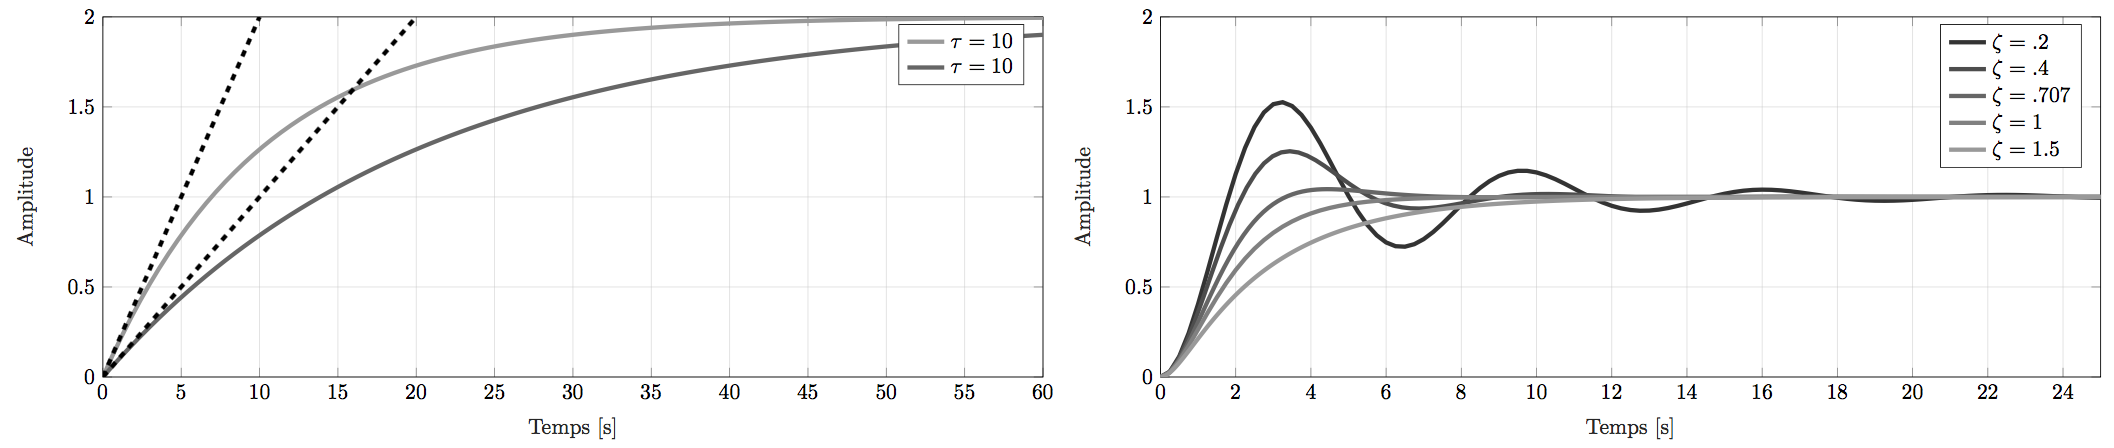
\includegraphics[width=\textwidth]{img/repind}
	\caption{Réponse indicielle de systèmess du premier ordre (gauche), % TODO fix legend
	avec en pointillé les tangentes à l'origine
	pour les systèmes du premier ordre,
	et de systèmes du second ordre (droite).}
	\label{fig:repind}
\end{figure}

Sur \matlab, les commandes \mintinline{Matlab}{step}
et \mintinline{Matlab}{lsim} permettent de calculer
une réponse indicielle et temporelle respectivement.

\section{Réponse fréquentielle et diagramme de Bode}
\subsection{Réponse fréquentielle}
\begin{mydef}
La \emph{réponse fréquentielle} de $G(s)$ est la représentation
de la fonction à valeur complexe, $\Gjw$,
avec $\omega$ une pulsation
associée à la fréquence $f$ telle que $\omega = 2 \pi f$,
et $\imagj^2 = -1$.
Le \emph{gain} ou \emph{module} de $\Gjw$,
noté $\abs{\Gjw}$,
ainsi que la \emph{phase}\footnote{$\angle z = \arctan(\Im(z)/\Re(z))$},
notée $\angle \Gjw$, sont représentés.
\end{mydef}

\subsection{Diagramme de Bode}
Le diagramme de Bode est une représentation graphique
de la réponse fréquentielle d'un système.
Il consiste en deux graphes:
\begin{itemize}
	\item le \emph{gain} en décibels (\si{\deci\bel})
	de la fonction de transfert, soit $20 \log_{10} \abs{\Gjw}$;
	\item la \emph{phase} de la fonction de transfert,
	exprimée en degrés, soit $\Gjw$.
\end{itemize}
Dans chacun des cas, l'axe des abscisses est à l'échelle logarithmique.

\subsubsection{Système du premier ordre}
La fonction de transfert du premier ordre type est donnée par
\begin{equation}
	\Gjw = \frac{k}{1 + \imagj \tau \omega}\,, \quad \tau, k > 0\,.
\end{equation}
L'amplitude et la phase de cette fonction de transfert sont
\begin{equation}
\begin{array}{rcl}
	\abs{\Gjw} & = & 20 \log_{10} \abs{\frac{k}{1 + \imagj \tau \omega}} = \frac{k}{1 + \sqrt{\tau^2 \omega^2}}\,, \\
	\angle \Gjw & = & - \arctan(\tau \omega)\,,
\end{array}
\end{equation}

On décompose l'étude en trois points:
\begin{itemize}
	\item Pour $0 < \tau \omega \ll 1$,
	\begin{equation}
	\begin{array}{rcrcl}
		\abs{\Gjw} & = & 20 \log_{10} \abs{\frac{k}{1 + \imagj \tau \omega}} & \simeq & 20 \log_{10} k \,, \\
		\angle \Gjw & = & -\arctan(\tau \omega)\Big|_{\tau \omega \ll 1} & \approx & \SI{0}{\degree}\,.
	\end{array}
	\end{equation}
	\item Pour $\omega = 1/\tau \iff \tau \omega = 1$,
	\begin{equation}
	\begin{array}{rcrclcl}
		\abs{\Gjw} & = & 20 \log_{10} \abs{\frac{k}{1 + \imagj \tau \omega}} & = & 20 \log_{10} k - 20 \log_{10} \sqrt{2} & \approx & 20 \log_{10} k - 3\,, \\
		\angle \Gjw & = & -\arctan(\tau \omega)\Big|_{\omega = 1/\tau} & \approx & -\SI{45}{\degree}\,.
	\end{array}
	\end{equation}
	\item Pour $\tau \omega \gg 1$,
	\begin{equation}
	\begin{array}{rcrcl}
		\abs{\Gjw} & = & 20 \log_{10} \abs{\frac{k}{1 + \imagj \tau \omega}} & \simeq & 20 \log_{10} k - 20 \log_{10} \tau \omega\,, \\
		\angle \Gjw & = & -\arctan(\tau \omega)\Big|_{\tau \omega \gg 1} & \approx & -\SI{90}{\degree}\,.
	\end{array}
	\end{equation}
\end{itemize}
Le tracé de l'amplitude est donc composé
de deux asymptotes sécantes en $\omega = 1/\tau$.
À gauche du point, le tracé est une droite horizontale
en $\abs{\Gjw} = 20 \log_{10} k$,
alors qu'à droite,
le tracé est une droite de pente $-\SI{20}{\deci\bel\per\dec}$.
Au point de cassure ($\omega = 1/\tau$),
la courbe réelle est à $-\SI{3}{\deci\bel}$
des droites asymptotiques\footnote{Ce qui revient
à une atténuation d'un facteur $\sqrt{2}$ de l'amplitude.}.

La \figuref{bode} illustre la réponse fréquentielle
de systèmes du premier et du deuxième ordre et son comportement asymptotique.

\begin{figure}[H]
	\centering
	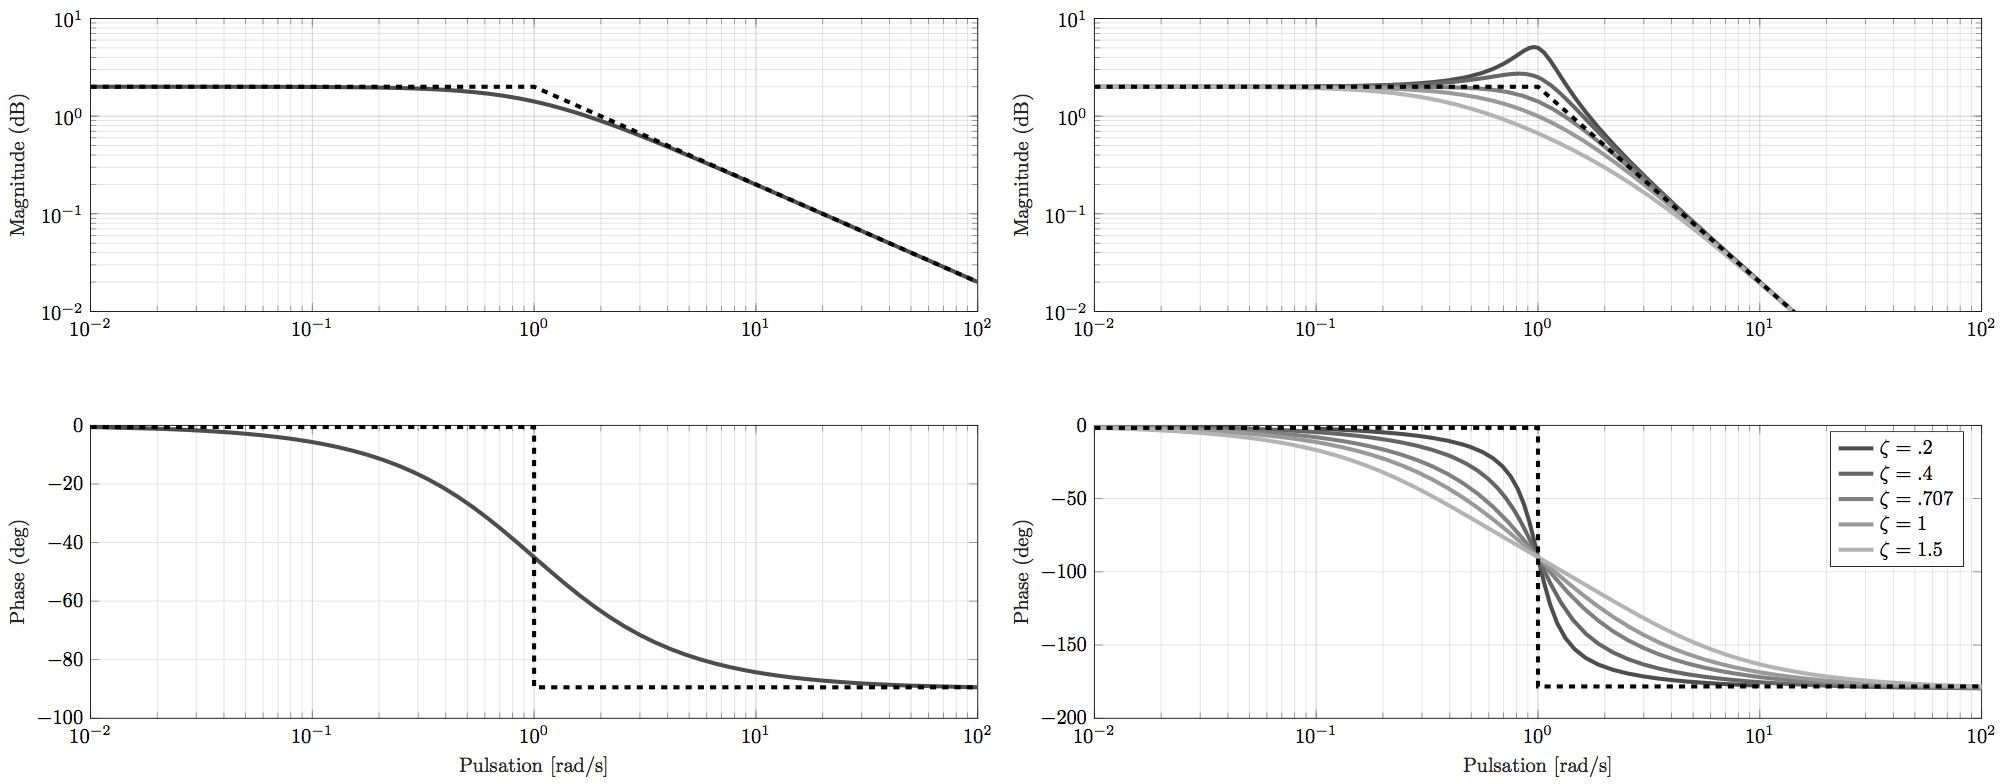
\includegraphics[width=\textwidth]{img/bode}
	\caption{Diagramme de Bode de systèmes du premier ordre (gauche)
	et de systèmes du second ordre (droite)
	avec le comportement asymptotique en pointillés.}
	% TODO fix axes
	\label{fig:bode}
\end{figure}

\begin{myrem}
	Pour un système du premier ordre avec un pôle strictement positif,
	le diagramme de bode est identique mais la phase change de signe.
\end{myrem}
\begin{myrem}
	Pour un système intégrateur avec la fonction de transfert $G(s) = k/s$,
	l'amplitude est une droite de pente $-\SI{20}{\deci\bel\per\dec}$
	qui vaut $\SI{0}{\deci\bel}$ pour $\omega = k$.
	La phase est constante et vaut $-\SI{90}{\degree}$.
\end{myrem}

\subsubsection{Système du second ordre}
La fonction de transfert du second ordre type est
\begin{equation}
	\Gjw = \frac{k}{1 + \imagj 2 \zeta \dfrac{\omega}{\omega_0} + \left( \dfrac{\imagj \omega}{\omega_0} \right)^2}\,.
\end{equation}
avec $0 \le \zeta \le 1$ le \emph{facteur d'amortissement}
et $k$ le \emph{gain}.
Le comportement asymptotique est encore décomposé en trois points:
\begin{itemize}
	\item Pour $\omega \to 0$,
	\begin{equation}
	\begin{array}{rcl}
		\abs{\Gjw} & \simeq & 20 \log_{10} k\,, \\
		\lim\limits_{\omega \to 0} \angle \Gjw & = & \SI{0}{\degree}\,.
	\end{array}
	\end{equation}
	\item Pour $\omega \to + \infty$,
	\begin{equation}
	\begin{array}{rcl}
		\abs{\Gjw} & \simeq & 20 \log_{10} k - 40 \log_{10} \left( \dfrac{\omega}{\omega_0} \right)\,, \\
		\lim\limits_{\omega \to +\infty} \angle \Gjw & = & -\SI{180}{\degree}\,.
	\end{array}
	\end{equation}
	\item Pour $\omega = \omega_0$,
	on trouve que $\angle\Gjw = -\SI{90}{\degree}$.
	Le comportement du gain
	au niveau de la \emph{fréquence de coupure} $\omega_0$
	varie en fonction de $\zeta$.
	\begin{itemize}
		\item Pour $\zeta = 1$,
		\begin{equation}
			\abs{\Gjw} \simeq 20 \log_{10} k - 20 \log_{10} 2 \approx 20 \log_{10} k - 6\,.
		\end{equation}
		\item Pour $\zeta > \sqrt{2}/2$, il n'y a pas de résonance.
		\item Pour $0 < \zeta < \sqrt{2}/2$,
		l'amplitude de $\Gjw$ est maximale
		à la pulsation de résonance $\omega_{\textnormal{r}}$,
		tel que
		\begin{equation}
		\begin{array}{rcl}
			\omega_{\textnormal{r}} & = & \omega_0 \sqrt{1 - 2 \zeta^2}\,, \\
			\abs{G(\imagj \omega_{\textnormal{r}})} & = & \frac{1}{2 \zeta \sqrt{1 - \zeta}}\,.
		\end{array}
		\end{equation}
	\end{itemize}
	Le tracé est donc l'intersection
	d'une droite horizontale en $20 \log k \si{\deci\bel}$
	avec une droite de pente $-\SI{40}{\deci\bel\per\dec}$
	à la pulsation $\omega_0$.
	La phase vaut $\SI{0}{\degree}$ avant en $\omega < \omega_0$
	et $-\SI{180}{\degree}$ en $\omega > \omega_0$.
	En $\omega = \omega_0$,
	$\angle\Gjw = -\SI{90}{\degree}$.
\end{itemize}

\subsection{Construction asymptotique du diagramme de Bode}
La fonction de transfert $G(s)$
d'un système d'ordre supérieur ou égal à un prend la forme
\begin{equation}
	G(s) = \frac{\prod\limits_{k = 1}^i N_k(s)}{\prod\limits_{k=1}^j D_k(s)}\,,
\end{equation}
avec $N_k(s)$ et $D_k(s)$ des polynômes du premier ou second ordre.
On a donc
\begin{equation}
	20 \log_{10} \abs{\Gjw} = \sum_k 20 \log_{10} \abs{N_k(\imagj \omega)} - \sum_k 20 \log_{10} \abs{D_k(\imagj \omega)}
\end{equation}
et
\begin{equation}
	\angle\Gjw = \angle N_k(\imagj \omega) - \angle D_k(\imagj \omega)\,.
\end{equation}
Les courbes de gain et de phase sont obtenues
en additionnant les courbes
des polynômes $N_k(\imagj \omega)$ et $D_k(\imagj \omega)$.
Les tracés asymptotiques sont obtenus par une étude de $\Gjw$ en
\begin{itemize}
	\item $\omega \to 0$ (très faible pulsation);
	\item $\omega \to +\infty$ (très forte pulsation);
	\item les pôles et zéros de $\Gjw$ (points de cassure).
\end{itemize}
La \tabref{asymp} reprend
les différentes variations de comportements asymptotiques.

Pour faire des diagrammes de bode sur \matlab,
on utilise la commande \mintinline{Matlab}{bode}.
\begin{table}[H]
\centering
\renewcommand\arraystretch{1.5}
\begin{tabular}{|c||cc|cc|cc|cc|}
	\hline
	Type/multiplicité & \multicolumn{2}{c|}{Pôle simple} & \multicolumn{2}{c|}{Zéro simple} & \multicolumn{2}{c|}{Pôles doubles} & \multicolumn{2}{c|}{Zéros doubles} \\
	Stabilité & Stable & Instable & Stable & Instable & Stable & Instable & Stable & Instable \\
	\hline
	\hline
	$\Delta \abs{\Gjw}$ & \multicolumn{2}{c|}{$-\SI{20}{\deci\bel\per\dec}$} & \multicolumn{2}{c|}{$+\SI{20}{\deci\bel\per\dec}$} & \multicolumn{2}{c|}{$-\SI{40}{\deci\bel\per\dec}$} & \multicolumn{2}{c|}{$+\SI{40}{\deci\bel\per\dec}$} \\
	$\Delta \angle\Gjw$ & $-\SI{90}{\degree}$ & $+\SI{90}{\degree}$ & $+\SI{90}{\degree}$ & $-\SI{90}{\degree}$ & $-\SI{180}{\degree}$ & $+\SI{180}{\degree}$ & $+\SI{180}{\degree}$ & $-\SI{180}{\degree}$ \\
	\hline
\end{tabular}
\caption{Table récapitulative des comportements asymptotiques.}
\label{tab:asymp}
\end{table}

\section{Linéarisation d'un système dynamique}
\subsection{Linéarisation d'un système dynamique non linéaire}
Soit le système de (\ref{eq:ssgen}).
L'objectif de la linéarisation consiste a remplacer ce système non linéaire,
autour du point d'équilibre $(\bar{x}, \bar{u}, \bar{v})$,
par un système linéaire à temps invariant.
\begin{mydef}
	Le point $(\bar{x}, \bar{u}, \bar{v})$ est un \emph{point d'équilibre}
	si et seulement si $f(\bar{x}, \bar{u}, \bar{v}) = 0$.
\end{mydef}
\begin{mydef}
	Le système linéarisé est exprimé
	en fonction des \emph{grandeurs variationnelles}
	définies autour du point d'équilibre $(\bar{x}, \bar{u}, \bar{v})$
	tel que $\tilde{x} \coloneqq x - \bar{x}$,
	$\tilde{u} \coloneqq u - \bar{u}$,
	$\tilde{v} \coloneqq v - \bar{v}$ et
	$\tilde{y} \coloneqq y - \bar{y}$, avec $y = h(\bar{x})$.
\end{mydef}

\subsubsection{Modèle du linéarisé tangent}
Le modèle linéarisé tangent du système non linéaire (\ref{eq:ssgen})
autour du point d'équilibre $\bar{\bm{x}} \coloneqq (\bar{x}. \bar{u}, \bar{v})$
est donné par
\begin{equation}
	\left\{
	\begin{array}{rcl}
		\dot{\tilde{x}}(t) & = & A \tilde{x}(t) + B \tilde{u}(t) + D \tilde{v}(t)\,, \\
		\\
		\tilde{y}(t) & = & C \tilde{x}(t)\,,
	\end{array}
	\right.
\end{equation}
avec
\begin{equation}
	A \coloneqq \left.\fpart{f}{x}\right|_{\bar{\bm{x}}}\,, \quad
	B \coloneqq \left.\fpart{f}{u}\right|_{\bar{\bm{x}}}\,, \quad
	D \coloneqq \left.\fpart{f}{v}\right|_{\bar{\bm{x}}}\,, \quad
	C \coloneqq \left.\fpart{h}{x}\right|_{\bar{x}}\,.
\end{equation}
Ce résultat est issu d'un développement de Taylor du premier ordre
des fonctions $f(x, u, v)$ et $h(x)$,
autour du point d'équilibre $\bar{\bm{x}}$.
\begin{equation}
	f(\bm{x}) \simeq f(\bar{\bm{x}}) + \left.\fpart{f}{x}\right|_{\bar{\bm{x}}} (x - \bar{x}) + \left.\fpart{f}{u}\right|_{\bar{\bm{x}}} (u - \bar{u}) + \left.\fpart{f}{v}\right|_{\bar{\bm{x}}} (v - \bar{v})
\end{equation}
et
\begin{equation}
	h(x) \simeq h(\bar{x}) + \left.\fdif{h}{x}\right|_{\bar{x}} (x - \bar{x})\,.
\end{equation}

\subsection{Stabilité d'un système linéarisé}
Pour un système non linéaire,
on ne parle plus de stabilité du système
mais de \emph{stabilité du point d'équilibre}.
La stabilité du point d'équilibre est obtenue en appliquant
les critères classiques de stabilité au système linéaire obtenu par
\emph{linéarisation du système non linéaire} autour de l'équilibre considéré.

Si $A$ n'admet que des valeurs propres à parties réelles strictement négatives,
plus au moins une valeur sur l'axe des imaginaires,
on ne peut pas conclure sur la stabilité du point d'équilibre.

\subsection{Exemples}
Les modèles de la \sectionref{models} peuvent être linéarisés.
Pour le pendule,
on trouve qu'à l'équilibre,
\begin{equation}
	\bar{x}_2 = 0 \quad \textnormal{et} \quad \sin \bar{x}_1 = 0 \implies \bar{x}_1 = 0 \quad \textnormal{ou} \quad \bar{x}_1 = \pi\,.
\end{equation}
Ces deux états d'équilibre correspondent respectivement
à la position stable avec le pendule en bas $(x_1 = 0)$
et la position instable avec le pendule en haut $(x_1 = \pi)$.

Dans le cas du bioréacteur,
on a trois états d'équilibre.
En effet, soit $\bar{X} = 0$,
ce qui correspond à l'absence de biomasse (lavage ou \emph{wash-out}),
soit $\mu = \frac{q}{V}$.
En regardant le graphe de la \figuref{growth},
on observe qu'il y a bien deux solutions à cette équation
(une dans la partie croissante
et l'autre dans la partie décroissante du graphe).

\section{Conditionnement de la commande}
\subsection{Retard pur}
Dans le domaine temporel, un \emph{retard pur} ou \emph{transport}
est modélisé par \(y(t) = u(t - \tau)\).
Dans le domaine fréquentiel,
on trouve \(\laplacian_t\left[ f(t - \tau) \right](s)
= \e^{-s \tau} \laplacian_t\left[f(t)\right](s)\).
On peut approximer ce retard soit par une série de Taylor
comme \(\e^{-s \tau} \approx 1 - s \tau\),
soit avec une approximation de Padé du premier ordre
comme \(\e^{-s \tau} = \frac{1 - s \tau/2}{1 + s \tau/2}\).
Sur \matlab, la fonction à utiliser est \mintinline{matlab}{pade}.

\section{Commande en boucle fermée}
\subsection{La boucle fermée}
Un système est dit en \emph{boucle fermée (BF)}
si le système est interconnecté dans un cycle comme dans la \figuref{olcl}.
À l'opposé, si nous cassons l'interconnexion, le système est dit en
\emph{boucle ouverte (BO)}.

\begin{figure}[H]
	\centering
	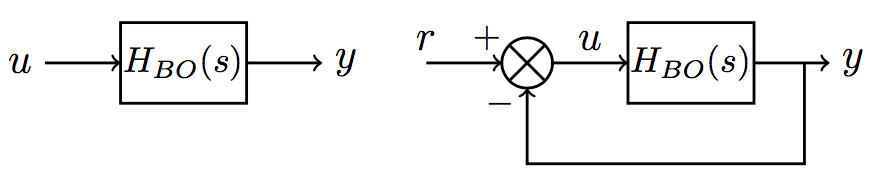
\includegraphics[width=0.7\textwidth]{img/olcl}
	\caption{À gauche, le système est en boucle ouverte,
	alors qu'à droite il est en boucle fermée.}
	\label{fig:olcl}
\end{figure}

Les systèmes en boucle fermée résultent
d'un retour de sortie dans le schéma de commande,
c'est-à-dire que la commande à un instant $t$
est une fonction du signal de référence $r(t)$ et de sortie $y(t)$.
Il peut prendre la forme d'une \emph{rétroaction}
et/ou d'un \emph{retour d'état}, avec ou sans \emph{compensateur}.

\subsection{Structure générale de commande}
\begin{figure}[H]
	\centering
	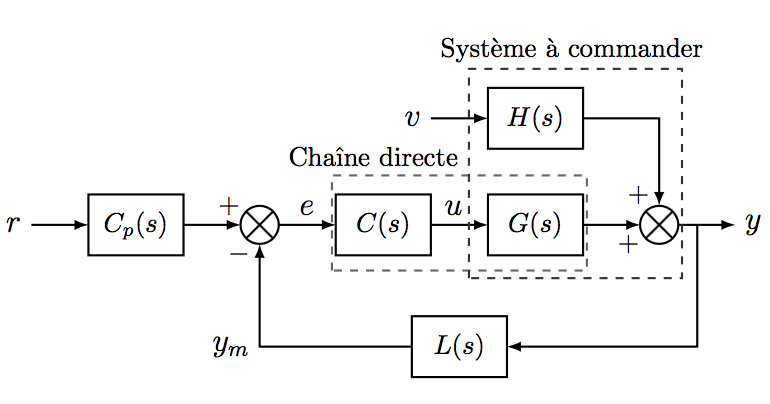
\includegraphics[width=0.7\textwidth]{img/command}
	\caption{Schéma-bloc de la structure de commande en boucle fermée.}
	\label{fig:command}
\end{figure}

La structure générale de commande d'un système modélisé par
la paire de fonctions de transfert $(G(s), H(s))$
est illustrée à la \figuref{command} où l'on retrouve les éléments suivants:
\begin{itemize}
	\item $r(t)$ est la \emph{consigne}\footnote{Parfois notée \(y^*(t)\).},
	un signal de référence que la \emph{sortie} $y(t)$ doit suivre.
	\item la \emph{sortie mesurée} $y_{\textnormal{m}}(t)$
	est acquise par l'intermédiaire d'un \emph{capteur},
	modélisé par la fonction de transfert $L(s)$.
	\item $e(t)$ est le signal d'\emph{erreur} entre
	la consigne filtrée et la mesure.
	\item $u(t)$ est la signal de \emph{commande} appliqué au système.
	\item $v(t)$ est la \emph{perturbation}, qui peut être connue ou non.
	\item $C_{\textnormal{p}}(s)$ et $C(s)$ sont les \emph{compensateurs}.
	$C_{\textnormal{p}}(s)$ est appelé \emph{pré-compensateur}
	en raison de son action directe sur le signal de référence.
	On peut écrire la loi de commande comme
	\(u(t) = C(s) [r(t) - y(t)]\)
\end{itemize}

Pour $r(t) = r$ constant, le problème de commande est un problème de régulation
(et/ou de réjection de perturbation).
Quand $r(t)$ est variable dans le temps,
on parle de problème de poursuite de trajectoire ou d'asservissement.

\subsection{Fonctions de transfert en boucle fermée}
Les entrées du système en boucle fermée sont $r(t)$ et $v(t)$,
alors que les signaux de sortie, que l'on souhaite observer
pour attester des performances du système en boucle fermée,
sont $y(t)$, $u(t)$ et $e(t)$.
On définit la fonction $S(s)$ telle que
\begin{equation}
	S(s) = \frac{1}{1 + C(s)G(s)L(s)}\,.
\end{equation}
Les fonctions de transfert suivantes
caractérisent le comportement du système bouclé
\begin{equation}
	\begin{pmatrix} y(t) \\ u(t) \\ e(t) \end{pmatrix} =
	\begin{pmatrix} T_{\textnormal{r}}(s) & T_{\textnormal{v}}(s) \\ U_{\textnormal{r}}(s) & U_{\textnormal{v}}(s) \\ E_{\textnormal{r}}(s) & E_{\textnormal{v}}(s) \end{pmatrix} \begin{pmatrix} r(t) \\ v(t) \end{pmatrix}\,,
\end{equation}
avec les fonctions de transfert entre les sorties et la référence
\begin{equation}
	T_{\textnormal{r}}(s) = C_{\textnormal{p}}(s) C(s) G(s) S(s)\,, \quad
	U_{\textnormal{r}}(s) = C_{\textnormal{p}}(s) C(s) S(s)\,, \quad
	E_{\textnormal{r}}(s) = C_{\textnormal{p}}(s) S(s)\,,
\end{equation}
et les fonctions de transfert vers la commande
\begin{equation}
	T_{\textnormal{v}}(s) = H(s) S(s)\,, \quad
	U_{\textnormal{v}}(s) = -H(s) C(s) L(s) S(s)\,, \quad
	E_{\textnormal{v}}(s) = -H(s) L(s) S(s)\,.
\end{equation}

\subsection{Retour d'état}
\begin{figure}[H]
	\centering
	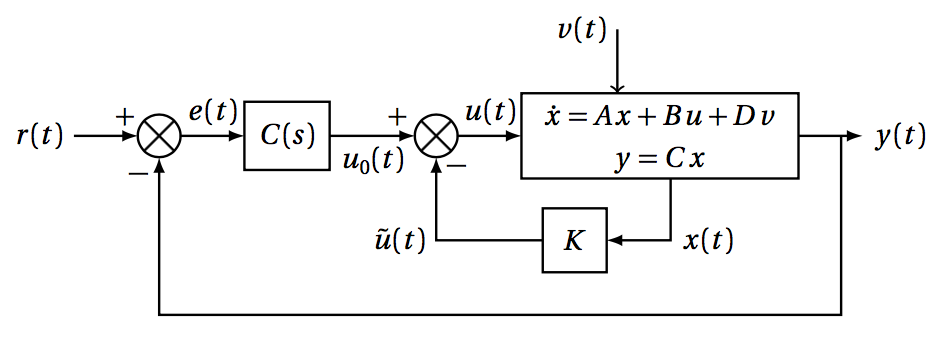
\includegraphics[width=\textwidth]{img/unitcommand.png}
	\caption{Schéma de commande avec retour d'état
	et boucle de rétroaction unitaire.}
\end{figure}
\begin{figure}[H]
	\centering
	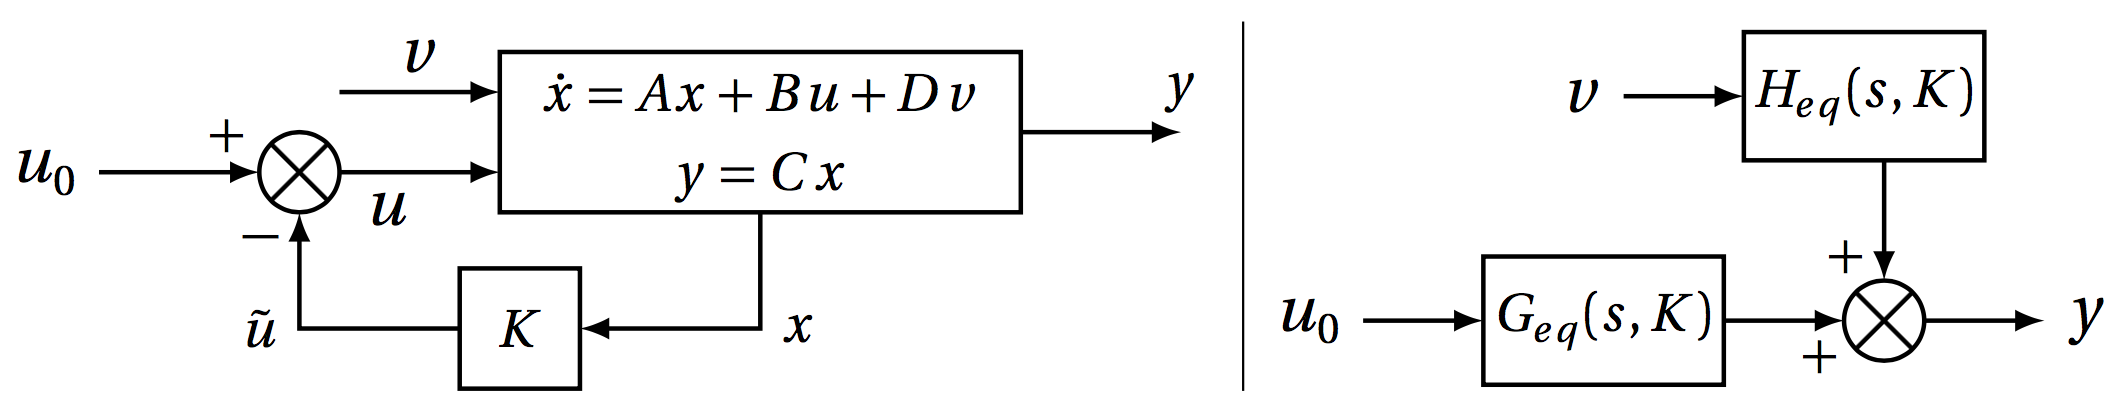
\includegraphics[width=\textwidth]{img/eqcommand.png}
	\caption{Commande par retour d'état (gauche)
	-- Fonctions de transfert équivalentes (droite).}
\end{figure}
Si la fonction de transfert en boucle ouverte
est donnée par \(G(s) = C(sI - A)^{-1}B\),
alors la fonction de transfert en boucle fermée
est donnée par \(\Geq(s) = C(sI - (A - BK))^{-1}B\).
En boucle fermée, la stabilité dépend donc
des valeurs propres de \(A - BK\).
Appelons ceux-ci \(\lambda_i\).
Le système est asymptotiquement stable
si et seulement si \(\Re\{\lambda_i\} < 0\), pour tout \(i\).

\subsection{Commande proportionnelle-intégrale-dérivée (PID)}
En plus des commandes proportionnelle et intégrale,
on rajoute un commande dérivée
avec une constante de temps de dérivation \(\taud > 0\) comme
\begin{equation}
	u = u^* + \kp (y^* - y) + \frac{\kp}{\taui} \int_0^t (y^* - y) \dif \tau + \kp \taud \fdif{}{t} (y^* - y)\,.
\end{equation}
On peut alors écrire la loi de commande comme
\begin{equation}
	\label{eq:commandlaw}
	C(s) = \kp \frac{1 + s \taui + s^2 \taui \taud}{s \taui}\,.
\end{equation}
On a ici fait deux simplifications;
l'équation complète est
\begin{equation}
	C(s) = \kp \left(\frac{1 + s \taui}{s \taui}\right) \left(\frac{1 + s \taud}{1 + s \alpha\taud}\right)\,,
\end{equation}
mais on considère en général que \(\taud \ll \taui\) et \(0 < \alpha \ll 1\).
Le régulateur PID fonctionne comme suit:
\begin{itemize}
	\item L'action proportionnelle (le gain \(\kp\)) permet
	de fixer la bande passante.
	\item L'action intégrale (le filtre \(\frac{1 + s\taui}{s \taui}\))
	annule l'erreur statique.
	\item L'action dérivée
	(le filtre à avance de phase \(\frac{1 + s \taud}{1 + s \alpha \taud}\))
	permet de fixer la marge de phase PM.
\end{itemize}

\subsubsection{Choix des paramètres}
Grâce à cette loi de commande,
il est possible de changer la dynamique d'un système.
On a \(T_{\textnormal{r}}(s) = \frac{C(s)G(s)}{1 + C(s)G(s)}\).
Avec une manipulation algébrique simple
(en posant \(T_{\textnormal{r}}(s) = G \dif g(s)\) et en remplaçant),
on trouve alors
\begin{equation}
	\label{eq:commandparam}
	C(s) = \frac{1}{G(s)} \frac{T_{\textnormal{r}}(s)}{1 - T_{\textnormal{r}}(s)}\,.
\end{equation}
On peut ainsi choisir une fonction de transfert en boucle fermée désirée,
étant donné la fonction de transfert en boucle ouverte.
Ensuite, on manipule l'expression obtenue pour \(C(s)\),
jusqu'à avoir quelque chose de la forme de \eqref{eq:commandlaw}.
On peut alors déterminer les paramètres à choisir \(\kp, \taui, \taud\)
afin d'obtenir la fonction de transfert en boucle fermée désirée.

\subsection{Système avec retard}
Dans le cas d'un système avec retard,
on pourrait essayer de faire la même chose pour faire disparaître celui-ci:
prenons un exemple pour illustrer.
\begin{myexem}
	Supposons qu'on connait
	la fonction de transfert en boucle ouverte d'un système avec retard:
	\(G(s) = K \frac{\e^{-\theta s}}{1 + s T_1}\).
	On souhaite appliquer un régulateur PI à ce système,
	afin d'obtenir une fonction de transfert en boucle fermée de la forme
	\(T_{\textnormal{r}} = \frac{\e^{-\theta s}}{1 + s T_2}\).

	On remplace dans \eqref{eq:commandparam}
	et on trouve
	\(C(s) = \frac{1 + s T_1}{K (-\e^{-\theta s}) + 1 + sT_2}\).
	On remarque donc que c'est impossible de faire disparaître le retard.
	Cependant, on peut approximer avec
	les séries de Taylor du premier ordre, pour obtenir
	\(C(s) \approx \frac{1 + s T_1}{K (s (\theta + T_2))}\).
	On observe qu'on peut factoriser cette loi de commande comme
	\(\frac{1}{K} \frac{T_1}{\theta + T_2} \frac{1 + s T_1}{s T_1}\),
	et on voit immédiatement que les paramètres du régulateur PI sont donc
	\(\taui = T_1\) et \(\kp = \frac{1}{K} \frac{T_1}{\theta + T_2}\).
\end{myexem}

Quelques règles de bonne pratique dans le cas de systèmes avec retard sont:
\begin{itemize}
	\item On essaie de prendre \(\kp \propto 1/K\),
	c'est-à-dire que le gain du régulateur est inversement proportionnel
	au gain du système.
	\item On essaie de prendre \(T_2 \in [T_1/10, T_1]\).
	\item Pour \(\theta > 0\),
	on essaie de prendre \(\kp \propto T_1/\theta\).
	\item Pour \(\theta > 0\),
	on essaie de prendre \(\taui \propto \theta/T_1\).
	\item Lorsqu'on ajoute la commande intégrale à un régulateur P,
	on diminue le gain \(\kp\).
	Lorsqu'on ajoute la commande dérivée à un régulateur PI,
	on augmente le gain \(\kp\).
\end{itemize}

\subsection{Paramétrisation de Youla-Ku\v{c}era}
La paramétrisation de Youla-Ku\v{c}era est une formule qui décrit
toutes les lois de commande stabilisantes pour un système donné,
comme une fonction d'un certain paramètre \(Q\).
\begin{figure}[H]
	\centering
	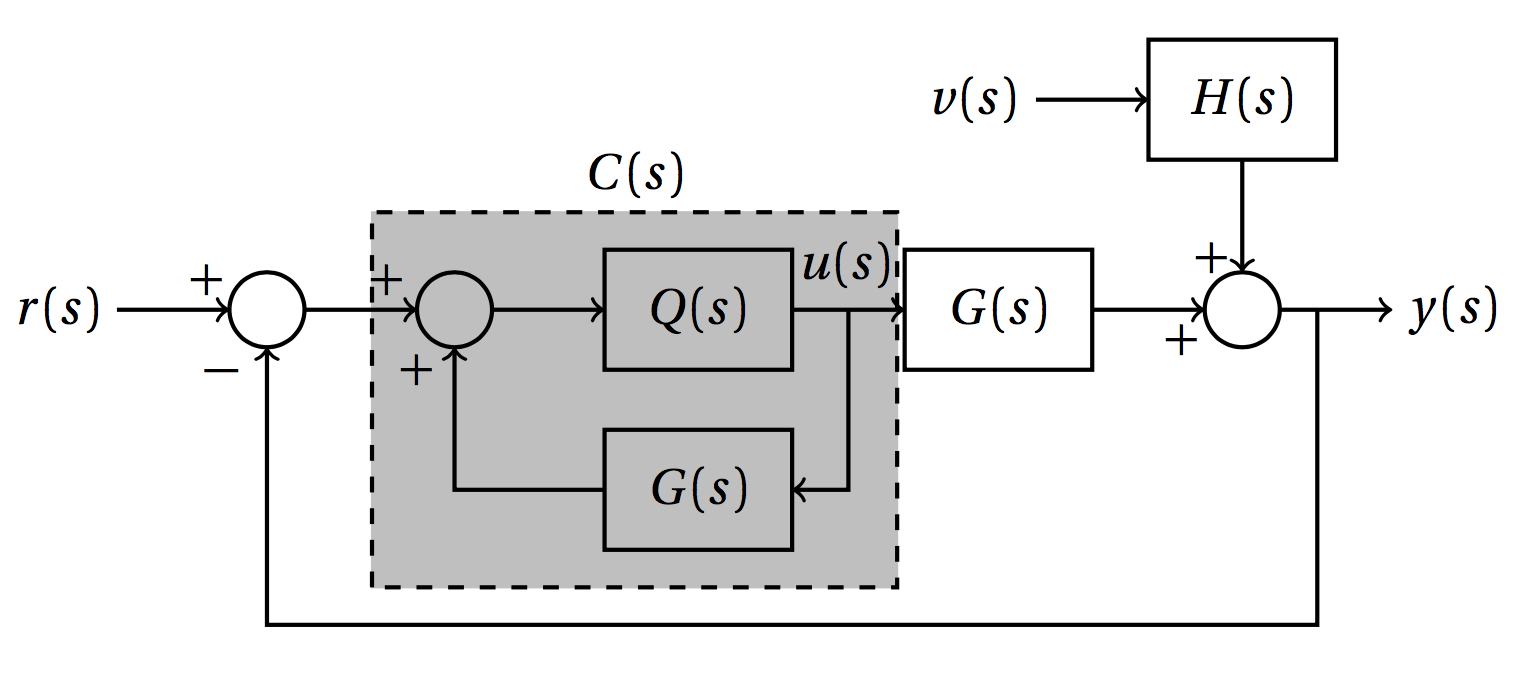
\includegraphics[width=0.7\textwidth]{img/youlakucera.png}
\end{figure}
Si \(G(s)\) est une fonction de transfert stable et propre,
alors le système est stable en boucle fermée,
avec \(Q(s)\) une fonction de transfert stable et propre.

On peut donc écrire
\begin{equation}
	C(s) = \frac{Q(s)}{1 - G(s)Q(s)}\,.
\end{equation}
Les fonctions de transfert entre les sorties et la référence deviennent alors
\begin{equation}
	T_{\textnormal{r}}(s) = Q(s) G(s)\,, \quad
	U_{\textnormal{r}}(s) = Q(s)\,,
\end{equation}
et les fonctions de transfert vers la commande
\begin{equation}
	T_{\textnormal{v}}(s) = H(s) (1 - Q(s)G(s))\,, \quad
	U_{\textnormal{v}}(s) = -H(s) Q(s)\,.
\end{equation}

\section{Analyse de stabilité en boucle fermée}
\subsection{Méthodes fréquentielles}
\subsubsection{Diagramme de Bode}
Afin d'utiliser le diagramme de Bode développé précédemment
comme un indicateur de stabilité,
on définit les marges de stabilité.
\paragraph{Marge de gain}
Pour trouver la marge de gain GM (aussi notée \(\gainm\)),
on cherche la fréquence \(\omega_\textnormal{L}\)
à laquelle la phase devient \(\SI{-180}{\degree}\):
\begin{equation}
	\arg\big(C(\imagj \omega_\textnormal{L}) \Geq(\imagj \omega_{\textnormal{L}})\big) = \SI{-180}{\degree}\,.
\end{equation}
On cherche alors le gain à cette fréquence, en décibels,
et on prend son opposé comme \emph{marge de gain}.
On peut donc écrire
\begin{equation}
	\textnormal{GM} = \gainm = -20 \log_{10}\abs{C(\imagj \omega_\textnormal{L}) \Geq(\imagj \omega_{\textnormal{L}})}\,.
\end{equation}

\paragraph{Marge de phase}
Pour trouver la marge de phase PM (aussi notée \(\phasem\)),
on cherche la fréquence de coupure \(\omega_{\textnormal{c}}\)
à laquelle le gain vaut \(\SI{0}{\deci \bel}\).
Sur le diagramme de gain de Bode,
c'est là où la fonction de transfert croise l'axe des abscisses:
\begin{equation}
	20 \log_{10}\abs{C(\imagj \omega_\textnormal{c}) \Geq(\imagj \omega_{\textnormal{c}})} = 0\,.
\end{equation}
On cherche alors la phase à cette fréquence, en degrés,
et on prend son antisupplémentaire comme \emph{marge de phase}.
On peut donc écrire
\begin{equation}
	\textnormal{PM} = \phasem = \SI{180}{\degree} + \arg\big(C(\imagj \omega_\textnormal{c}) \Geq(\imagj \omega_{\textnormal{c}})\big)\,.
\end{equation}

\paragraph{Marge de stabilité absolue}
La \emph{marge de stabilité absolue (ou marge de module)},
notée \(\sigma_\textnormal{M}\),
est la distance minimale entre le point \((-1, 0)\)
et la courbe gain/phase sur le plan complexe.
\begin{equation}
	\sigma_{\textnormal{M}} = \inf_{\omega \ge 0} 20 \log_{10} \abs{1 + C(\imagj \omega) G(\imagj \omega)}\,.
\end{equation}

Pour analyser la stabilité avec ces marges,
on se donne l'intuition que tant que les marges sont strictement positives,
le système est stable.
On peut donc décider comme suit:
\begin{itemize}
	\item \(\omega_{\textnormal{c}} < \omega_{\textnormal{L}} \iff \gainm, \phasem > 0\), et donc le système est stable.
	\item \(\omega_{\textnormal{c}} = \omega_{\textnormal{L}} \iff \gainm, \phasem = 0\), et donc le système est en limite de stabilité.
	\item \(\omega_{\textnormal{c}} > \omega_{\textnormal{L}} \iff \gainm, \phasem < 0\), et donc le système est instable.
\end{itemize}
Sur \matlab, la fonction à utiliser est \mintinline{matlab}{margin},
qui permet de visualiser facilement les fréquences et les marges.

\subsubsection{Critère de stabilité de Nyquist}
\begin{mydef}[Fonction holomorphe]
	Une \emph{fonction holomorphe} est une fonction à valeurs complexes,
	définie et dérivable en tout point
	d'un sous-ensemble ouvert du plan complexe \(\C\).
	Toute fonction holomorphe est \emph{analytique}.
\end{mydef}
\begin{mydef}[Fonction méromorphe]
	Une \emph{fonction méromorphe} est une fonction holomorphe
	dans tout le plan complexe, sauf éventuellement
	sur un ensemble de points isolés
	dont chacun est un pôle pour la fonction.
\end{mydef}
\begin{mytheo}[Principe de l'argument---Cauchy, 1831]
	Si un contour \(\Gamma_s\) dans le plan \(s\) complexe
	encercle \(Z\) zéros et \(P\) pôles d'une fonction méromorphe \(F(s)\)
	et ne passe pas par une racine de \(F(s)\),
	si le parcours est dans le sens horaire,
	alors le contour correspondant \(\Gamma_{F(s)} = F(\Gamma_s)\)
	dans le plan \(F(s)\)
	encercle l'origine \(N = Z - P\) fois dans le sens horaire.
\end{mytheo}
\begin{myrem}
	Des encerclements dans le sens opposé sont comptés comme négatifs.
	On prend donc des encerclements positifs dans le sens horaire
	et négatifs dans le sens anti-horaire.
\end{myrem}

On construit alors le contour de Nyquist \(\Gamma_s\),
qui encercle le plan complexe de droite, comme suit:
\begin{itemize}
	\item un chemin montant le long de l'axe imaginaire,
	de \(0 - \imagj \omega\) à \(0 + \imagj \omega\);
	\item un arc semicirculaire, de rayon \(r \to +\infty\),
	qui commence en \(0 + \imagj \omega\)
	et qui passe en sens horaire à \(0 - \imagj \omega\).
\end{itemize}
Posons \(n_I\) le nombre de pôles instables de \(C(s)\Geq(s)\),
la fonction de transfert en boucle ouverte.
On observe que si on pose \(F(s) = C(s)\Geq(s)\),
alors le nombre d'encerclements \(N\)
du point \(-1 + \imagj 0\) par \(\Gamma_{F(s)}\)
dans le sens anti-horaire lorsqu'elle est parcourue
dans le sens \(0 \xrightarrow{\omega} +\infty\) doit être égal à \(n_I\)
pour une fonction de transfert
en boucle fermée \(T_{\textnormal{r}}(s)\) stable.
En résumé, \(n_I = N\) si et seulement si \(T_{\textnormal{r}}(s)\) est stable.

\begin{myrem}
Dans le cas où on a des pôles sur l'axe imaginaire,
il faut légèrement modifier le contour de Nyquist:
supposons qu'on ait un pôle en \(0 + \imagj \omega\);
il faut alors construire un arc semicirculaire de rayon \(r \to 0\)
autour de \(0 + \imagj \omega\),
qui commence en \(0 + \imagj (\omega - r)\)
et qui passe en \(0 + \imagj (\omega + r)\)
dans le sens anti-horaire, encerclant le pôle posant problème.
\end{myrem}

Comme le critère de stabilité de Nyquist
ne nécéssite pas le calcul des racines proprement dit
(il suffit de connaître le nombre de racines dans le demi-plan de droite),
on peut également l'appliquer aux systèmes non rationnels,
avec des retards par exemple.

Avec le critère de stabilité de Nyquist,
on peut également calculer les marges de stabilité.
La marge de gain est le facteur avec lequel on doit multiplier le gain
tel que la courbe de Nyquist passe par \(-1 + \imagj 0\).

On définit la marge de stabilité absolue, c'est-à-dire la marge de module, comme
\begin{equation}
	\sigma_{\textnormal{M}} = \inf_\omega 20 \log_{10}\abs{1 + C(\imagj \omega) \Geq(\imagj \omega)}\,.
\end{equation}
On l'exprime toujours en décibels.
Conversement, la marge de phase est l'angle duquel on peut tourner
le diagramme de Nyquist avant de passer par \(-1 + \imagj 0\).

Sur \matlab, on utilise la fonction \mintinline{matlab}{nyquist}
pour dessiner le diagramme de Nyquist.

\subsection{Analyse du lieu des racines -- \emph{root locus}}
Soit une fonction de transfert en boucle ouverte de la forme \(C(s)G(s)\),
supposée connue et avec
\begin{align}
	C'(s)G(s) &= \frac{N(s)}{D(s)} = \frac{\prod_{i=1}^m (s - z_i)}{\prod_{i=1}^n (s = p_i)}\,.
	\intertext{En boucle fermée,
	on trouve alors que les pôles sont les racines du dénominateur de}
	1 + C(s)G(s) &= 1 + \underbrace{\kp C'(s)}_{C(s)} G(s)\\
	&= 1 + \kp \frac{N(s)}{D(s)}\\
	&= \frac{D(s) + \kp N(s)}{D(s)}\,,
\end{align}
où \(\kp \in \R\) est le gain du compensateur.
\begin{mydef}
	Le \emph{lieu des racines} est une représentation dans le plan complexe
	des pôles de la fonction de transfert en boucle fermée,
	pour un gain \(\kp\) variant de \(0\) à \(+\infty\).
\end{mydef}
\begin{mynota}
	Par convention, les zéros sont indiqués par des cercles,
	alors que les pôles sont indiqués par des croix.
\end{mynota}
\begin{myrem}
	Pour un système avec un zéro instable en \(b\),
	on factorise la fonction de transfert par \(-b\).
	Ainsi,
	le gain \(\kp\) devient le gain fictif \(-\kp b\)
	que l'on fait varier entre \(0\) et \(-\infty\).
\end{myrem}

\subsubsection{Éléments de construction du lieu des racines}
Les règles suivantes permettent de comprendre, tracer et interpréter
un lieu des racines.
\begin{enumerate}
	\item Le lieu possède \(n\) branches,
	dont les \(n\) points de départ \(\kp = 0\)
	sont les racines de \(D(s)\) (les pôles en BO),
	et les points d'arrivée \(\kp \to +\infty\)
	sont les \(m\) racines de \(N(s)\) (les zéros en BO)
	et \(n-m\) asymptotes.
	\item \emph{Dans le cas sans zéro instable},
	les \(n-m\) points à l'infini sont orientés suivant les asymptotes
	d'angle \(\frac{2k+1}{n-m} \pi\), pour \(k = 0, \ldots, n-m-1\).
	\emph{Dans le cas avec un zéro instable},
	les asymptotes sont d'angle
	\(\frac{2k}{n-m} \pi\), pour \(k = 0, \ldots, n-m-1\).
	Les asymptotes s'intersectent au point
	\begin{equation}
		P = \frac{1}{n-m} \left(\sum_{j=1}^n p_j - \sum_{i=1}^m z_i\right)\,.
	\end{equation}
	\item \emph{Dans le cas sans zéro instable},
	les segments de l'axe réel qui sont à gauche
	d'un nombre impair de racines de \(D(s)\) ou \(N(s)\)
	appartiennent au lieu des racines si \(\kp \ge 0\).
	\emph{Dans le cas avec un zéro instable},
	les segments de l'axe réel qui sont à gauche
	d'un nombre pair de racines de \(D(s)\) ou \(N(s)\)
	appartiennent au lieu des racines si \(\kp \le 0\).
	\item Le lieu des racines est symétrique par rapport à l'axe réel.
	\item Les points de séparation de l'axe des réels
	sont des racines doubles et sont solutions de
	\begin{equation}
		N(s) \fdif{D(s)}{s} - D(s) \fdif{N(s)}{s} = 0\,.
	\end{equation}
\end{enumerate}

Sur \matlab, la commande à utiliser est \mintinline{matlab}{rlocus}.

\section{Commande linéaire quadratique (LQ)}
\subsection{Critère de minimisation}
La commande linéaire quadratique est une commande de référence,
qui n'est pas toujours optimale mais qui permet de se faire une idée.
Elle correspond au choix d'une commande \(u(t)\)
telle que \(u(t)\) soit la solution linéaire du problème
de la minimisation d'une fonctionnelle quadratique \(J\), définie comme suit:
\begin{equation}
	J = \min_{u(t)} \left[ \int_0^{+\infty} \left(x^T Q_x x + u^T Q_u u\right) \dif t\right]\,,
\end{equation}
où \(Q_x = Q_x^T \succeq 0\) et \(Q_u = Q_u^T \succ 0\).
Ce choix provient du fait
que l'on veut pénaliser les variations de l'état \(x(t)\) par rapport à zéro
et pénaliser les variations de la commande,
avec un certain facteur d'importance
(donné par \(Q_x\) et \(Q_u\), respectivement).

\subsection{Solution du problème de minimisation}
\begin{mytheo}
	Si \((A, B)\) est stabilisable et si \((Q_x, A)\) est détectable,
	alors
	\begin{itemize}
		\item il existe une solution unique \(S = S^T \succeq 0\)
		de l'équation de Riccati algébrique
		\begin{equation}
			A^T S + SA + S B Q_u^{-1} B^T S + Q_x = 0\,;
		\end{equation}
		\item \(A - BQ_u^{-1}S\) est asymptotiquement stable.
	\end{itemize}
\end{mytheo}
Pour pouvoir appliquer la commande LQ,
il suffit donc d'avoir un système détectable
(et donc pas nécessairement commandable,
quoique la commandabilité est nécessaire pour les garanties de convergence).
La condition \((A, B)\) stabilisable garantit qu'il existe une commande \(u\)
telle que la fonctionnelle de coût soit finie pour tout état \(x\).
Pour le voir, il suffit de se rappeler l'expansion
avec l'exponentielle matricielle de \eqref{eq:matrixexponential}
et de remplacer dans la fonction de coût \(J\).
En effet, si on n'a pas la stabilisabilité,
alors cette intégrale ne peut être finie.

Si au lieu d'avoir \((A, B)\) stabilisable et \((Q_x, A)\) détectable,
on a \((A, B, C)\) stabilisable/détectable,
alors dans la fonctionnelle à minimiser, on doit remplacer
\(x^T Q_x x\) par \(y^T y = x^T C^T C x\).
Cela revient à avoir \(Q_x =  C^T C\).
On pénalise alors la sortie, plutôt que l'état proprement dit.
Ici, \((A, B, C)\) stabilisable/détectable
(avec \(A \in \Rnn, B \in \Rnm\) et \(C \in \R^{q \times n}\)) signifie
qu'il existe un gain fixe \(K \in \R^{m \times q}\) tel que
\(A - B K C\) soit une matrice de Hurwitz.
C'est équivalent à avoir \((A, B)\) stabilisable
et \((C, A)\) détectable.

On peut alors résoudre ce problème de minimisation.
On commence par mettre l'équation de Riccati sous une forme équivalente:
\begin{align}
	Q_x &= S B Q_u^{-1} B^T S - A^T S - S A\\
	\iff x^T Q_x x &= x^T (S B Q_u^{-1} B^T S) x - x^T (A^T S - S A) x\\
	\iff x^T Q_x x + u^T Q_u u &= x^T (S B Q_u^{-1} B^T S) x + u^T Q_u u - x^T (A^T S - S A) x\,.\\
	\intertext{Ensuite, on remarque que \(SBQ_u^{-1} B^T S = SBQ_u^{-1} Q_u Q_u^{-1} B^T S\).
	On peut donc grouper comme suit
	(en se rappelant que \(Q_u\) est symétrique):}
	&= \begin{multlined}[t]
	\left( Q_u^{-1} B^T S x + u\right)^T Q_u \left(Q_u^{-1} B^T S x + u\right) \\
	- \underbrace{\left(x^T S B Q_u^{-1} Q_u u + u^T Q_u Q_u^{-1} B^T S x + x^T (A^T S + S A) x\right)}_{x^T S (B u + Ax) + (B u + Ax)^TSx = x^T S \dot{x} + \dot{x}^T S x = \frac{\dif}{\dif t}(x^T S x)}
	\end{multlined}\\
	\implies J &= \int_0^{+\infty} \left( Q_u^{-1} B^T S x + u\right)^T Q_u \left(Q_u^{-1} B^T S x + u\right) \dif t - \int_0^{+\infty} \frac{\dif}{\dif t} (x^T S x) \dif t\,.
	\intertext{Cette deuxième intégrale est égale à \(x_0^T S x_0\),
	qui est orthogonal à \(u(t)\)\footnote{Et ne peut donc pas
	être influencé par \(u\).},
	sous l'hypothèse raisonnable\footnote{Comme le système
	est stable en boucle fermée.} que
	\(\lim_{t \to +\infty} x(t) = 0\).
	La commande \(u(t)\) qui minimise \(J\) est donc}
	u(t) &= - Q_u^{-1} B^T S x(t)\,.
\end{align}
Avec un retour d'état donné par \(u(t) = - Kx(t)\),
on prend donc
\begin{equation}
	K = Q_u^{-1} B^T S\,.
\end{equation}
Sur \matlab, on utilise la fonction \mintinline{matlab}{lqr}.

\appendix
\section{Modèles}
\label{sec:models}
Les modèles suivants sont utilisés au long de l'année
pour expliquer les différents concepts.
\subsection{Pendule}
\noindent\begin{minipage}[c]{0.45\textwidth}
	\centering
	\begin{tikzpicture}
		% save length of g-vector and theta to macros
		\pgfmathsetmacro{\Gvec}{1.5}
		\pgfmathsetmacro{\myAngle}{30}

		\coordinate (centro) at (0,0);
		\draw[dashed,gray,-] (centro) -- ++ (0,-3) node (mary) [black,below]{};
		\draw[thick] (centro) -- ++(270+\myAngle:3)
			coordinate (bob)
			node[below right]{$m$}
			node[midway, right] {$\ell$};
		\pic [draw, ->, "$\theta$", angle eccentricity=1.5] {angle = mary--centro--bob};
		\filldraw [fill=black!40,draw=black] (bob) circle[radius=0.15];
	\end{tikzpicture}
\end{minipage}%
\begin{minipage}[c]{0.55\textwidth}
	On modélise le pendule par l'équation
	\begin{equation}
		m \ell \ddot{\theta} + mg \sin \theta + k \ell \dot{\theta} = 0\,.
	\end{equation}
	La représentation d'état est donc
	\begin{equation}
		\begin{pmatrix} x_1 = \theta \\ x_2 = \dot{\theta} \end{pmatrix} \iff
		\left\{
		\begin{array}{rcl}
			\dot{x}_1 & = & x_2\,, \\
			\\
			\dot{x}_2 & = & \dfrac{g}{\ell} \sin x_1 - \dfrac{k}{m} x_2\,.
		\end{array}
		\right.
	\end{equation}
	Cette équation est non linéaire à cause du $\sin \theta$.
\end{minipage}
\subsection{Bioréacteur}
\noindent\begin{minipage}[c]{0.45\textwidth}
	\centering
	\begin{figure}[H]
	\centering
	\begin{tikzpicture}[scale=0.7]
	\begin{axis}[
		xlabel={$S$},
		ylabel={$\mu(S)$},
		ylabel style={rotate=-90}
	]
		\addplot [
			black,
			domain=0:25,
			samples=201,
		]
		{5*x/(5+x+x*x/2)};
	\end{axis}
	\end{tikzpicture}
	\caption{Fonction de croissance.}
	\label{fig:growth}
	\end{figure}
\end{minipage}%
\begin{minipage}[c]{0.55\textwidth}
	Le bioréacteur est un système non linéaire
	qui représente la transformation
	de substrat $S$ en biomasse $X$.
	Sa représentation d'état est la suivante.
	\begin{equation}
		\left\{
		\begin{array}{rcl}
			\dot{X} & = & \left(\mu(S) - \dfrac{q}{V}\right) X\,, \\
			\\
			\dot{S} & = & -k \mu(S) X + \dfrac{q}{V} (S_{\textnormal{in}} - S)\,.
		\end{array}
		\right.
	\end{equation}

	La fonction de croissance $\mu(S)$ est donnée par l'équation
	\begin{equation}
		\mu(S) = \mu^* \frac{S}{k_S + S + \dfrac{S^2}{k}}\,.
	\end{equation}
	Elle montre comment croît la biomasse
	en fonction de la quantité de substrat disponible.
	Elle est montrée à la \figuref{growth}.
\end{minipage}

\section{Inverse d'une matrice}
\label{ann:inv}
En général, l'inverse d'une matrice $A$ est donné par
\[
A^{-1} = \frac{\adj(A)^T}{\det{A}}\,.
\]
Dans le cas d'une matrice $2 \times 2$, on a donc
\[
A = \begin{pmatrix} a_{11} & a_{12} \\ a_{21} & a_{22} \end{pmatrix}
\iff A^{-1} = \frac{1}{a_{11}a_{22} - a_{21}a_{12}} \begin{pmatrix} a_{22} & -a_{12} \\ -a_{21} & a_{11} \end{pmatrix}\,.
\]

\end{document}
